%
% chapter.tex
%
% (c) 2020 Prof Dr Andreas Müller, Hochschule Rapperswil
%
\chapter{Matrizengruppen
\label{buch:chapter:matrizengruppen}}
\lhead{Matrizengruppen}
\rhead{}
Matrizen können dazu verwendet werden, Symmetrien von geometrischen oder
physikalischen Systemen zu beschreiben.
\index{Symmetrie}%
\index{physikalisches System}%
Neben diskreten Symmetrien wie zum Beispiel Spiegelungen gehören dazu
\index{diskrete Symmetrie}%
\index{Symmetrie!diskret}%
\index{Spiegelung}%
auch kontinuierliche Symmetrien wie Translationen oder Invarianz einer
\index{kontinuierliche Symmetrie}%
\index{Symmetrie!kontinuierlich}%
\index{Translation}%
physikalischen Grösse über die Zeit.
Solche Symmetrien müssen durch Matrizen beschrieben werden können,
die auf stetige oder sogar differenzierbare Art von der Zeit abhängen.
Die Menge der Matrizen, die zur Beschreibung solcher Symmetrien benutzt
werden, muss also eine zusätzliche Struktur haben, die ermöglicht, 
sinnvoll über Stetigkeit und Differenzierbarkeit bei Matrizen
\index{Stetigkeit}%
\index{Differenzierbarkeit}%
zu sprechen.

Die Menge der Matrizen bilden zunächst eine Gruppe,
die zusätzliche differenzierbare Struktur macht daraus
eine sogenannte Lie-Gruppe.
\index{Lie-Gruppe}%
Die Ableitungen nach einem Parameter sind nicht mehr Gruppenelemente,
wie man nach allem, was man in der Analysis-Grundvorlesung
gelernt hat, vielleicht erwarten würde.
Sie liegen in der sogenannten Lie-Algebra,
einer Matrizen-Algebra mit dem antisymmetrischen
\index{Lie-Algebra}%
\index{antisymmetrisch}%
Lie-Klammer-Produkt $[A,B]=AB-BA$, auch Kommutator genannt.
\index{Lie-Klammer}%
\index{Kommutator}%
Lie-Gruppe und Lie-Algebra sind eng miteinander verknüpft,
so eng, dass sich die meisten Eigenschaften der Gruppe aus den Eigenschaften
der Lie-Gruppe aus der Lie-Algebra ableiten lassen.
Die Verbindung wird hergestellt durch die Exponentialabbildung.
Ziel dieses Kapitels ist, die Grundzüge dieses interessanten 
Zusammenhangs darzustellen.

%
% symmetrien.tex -- Geometrische Beschreibung von Symmetrien, O(n), SO(n),
%                   Spiegelungen
%
% (c) 2020 Prof Dr Andreas Müller, Hochschule Rapperswil
%
\section{Symmetrien
\label{buch:section:symmetrien}}
\rhead{Symmetrien}
Der geometrische Begriff der Symmetrie meint die Eigenschaft eines
geometrischen Objektes, dass es bei einer Bewegung auf sich selbst
abgebildet wird.
Das Wort stammt aus dem altgriechischen, wo es {\em Gleichmass}
bedeutet.
Spiegelsymmetrische Objekte zeichnen sich zum Beispiel dadurch aus,
dass Messungen von Strecken die gleichen Werte ergeben wie die Messungen
der entsprechenden gespiegelten Strecken (siehe auch
Abbildung~\ref{buch:lie:bild:castlehoward}, was die Herkunft des
Begriffs verständlich macht.
\begin{figure}
\centering
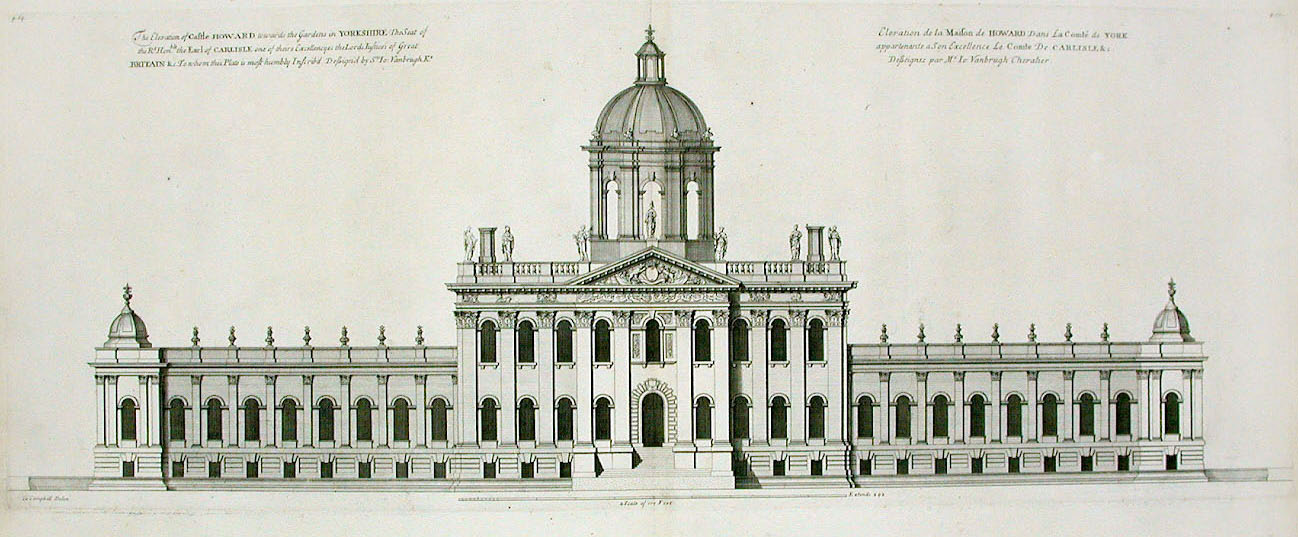
\includegraphics[width=\textwidth]{chapters/60-gruppen/images/castle.jpeg}
\caption{Das Castle Howard in Yorkshire war in dieser ausgeprägt symmetrischen
Form geplant, wurde dann aber in modifizeirter Form gebaut.
Messungen zwischen Punkten in der rechten Hälfte des Bildes
ergeben die gleichen Werte wie Messungen entsprechenden Strecken
in der linken Hälfte, was den Begriff Symmetrie rechtfertigt.
\label{buch:lie:bild:castlehoward}}
\end{figure}
In der Physik wird dem Begriff der Symmetrie daher auch eine erweiterte
Bedeutung gegeben.
Jede Transformation eines Systems, welche bestimmte Grössen nicht
verändert, wird als Symmetrie bezeichnet.
Die Gesetze der Physik sind typischerweise unabhängig davon, wo man den
den Nullpunkt der Zeit oder das räumlichen Koordinatensystems ansetzt,
eine Transformation des Zeitnullpunktes oder des Ursprungs des
Koordinatensystems ändert daher die Bewegungsgleichungen nicht, sie ist
eine Symmetrie des Systems.

Umgekehrt kann man fragen, welche Symmetrien ein System hat.
Da sich Symmetrien zusammensetzen und umkehren lassen, kann man in davon
ausgehen, dass die Symmetrietransformationen eine Gruppe bilden.
Besonders interessant ist dies im Falle von Transformationen, die
durch Matrizen beschrieben weren.
Eine unter der Symmetrie erhaltene Eigenschaft definiert so eine
Untergruppe der Gruppe $\operatorname{GL}_n(\mathbb{R})$ der
invertierbaren Matrizen.
Die erhaltenen Eigenschaften definieren eine Menge von Gleichungen,
denen die Elemente der Untergruppe genügen müssen.
Als Lösungsmenge einer Gleichung erhält die Untergruppe damit eine
zusätzliche geometrische Struktur, man nennt sie eine differenzierbare
Mannigfaltigkeit.
Dieser Begriff wird im Abschnitt~\ref{buch:subsection:mannigfaltigkeit}
eingeführt.
Es wird sich zum Beispiel zeigen, dass die Menge der Drehungen der
Ebene mit den Punkten eines Kreises parametrisieren lassen,
die Lösungen der Gleichung $x^2+y^2=1$ sind.

Eine Lie-Gruppe ist eine Gruppe, die gleichzeitig eine differenzierbare
Mannigfaltigkeit ist.
Die Existenz von geometrischen Konzepten wie Tangentialvektoren
ermöglicht zusätzliche Werkzeuge, mit denen diese Gruppe untersucht
und verstanden werden können.
Ziel dieses Abschnitts ist, die Grundlagen für diese Untersuchung zu
schaffen, die dann im Abschnitt~\ref{buch:section:lie-algebren}
durchgeführt werden soll.

\subsection{Algebraische Symmetrien
\label{buch:subsection:algebraische-symmetrien}}
Mit Matrizen lassen sich Symmetrien in einem geometrischen Problem
oder in einem physikalischen System beschreiben.
Man denkt dabei gerne zuerst an geometrische Symmetrien wie die
Symmetrie unter Punktspiegelung oder die Spiegelung an der $x_1$-$x_2$-Ebene,
wie sie zum Beispiel durch die Abbildungen
\[
\mathbb{R}^3\to\mathbb{R}^3 : x\mapsto -x
\qquad\text{oder}\qquad
\mathbb{R}^3\to\mathbb{R}^3 :
\begin{pmatrix}x_1\\x_2\\x_3\end{pmatrix}
\mapsto
\begin{pmatrix}-x_1\\x_2\\x_3\end{pmatrix}
\]
dargestellt werden.
Beide haben zunächst die Eigenschaft, dass Längen und Winkel und damit
das Skalarprodukt erhalten sind.
Diese Eigenschaft allein erlaubt aber noch nicht, die beiden Transformationen
zu unterscheiden.
Die Punktspiegelung zeichnet sich dadurch aus, das alle Geraden und alle
Ebenen durch den Ursprung auf sich selbst abgebildet werden.
Dies funktioniert für die Ebenenspiegelung nicht, dort bleibt nur die
Spiegelungsebene (die $x_1$-$x_2$-Ebene im vorliegenden Fall) und
ihre Normale erhalten.
Die folgenden Beispiele sollen zeigen, wie solche Symmetriedefinitionen
auf algebraische Bedingungen an die Matrixelemente führen.

Zu jeder Abbildung $f\colon\mathbb{R}^n\to\mathbb{R}^n$, unter der 
ein geometrisches Objekt in $\mathbb{R}^n$ symmetrisch ist, können wir
sofort weitere Abbildungen angeben, die ebenfalls Symmetrien sind.
Zum Beispiel sind die iterierten Abbildungen $f\circ f$, $f\circ f\circ f$
u.~s.~w., die wir auch $f^n$ mit $n\in\mathbb{N}$ schreiben werden,
ebenfalls Symmetrien.
Wenn die Symmetrie auch umkehrbar ist, dann gilt dies sogar für alle
$n\in\mathbb{Z}$.
Wir erhalten so eine Abbildung
$\varphi\colon \mathbb{Z}\to \operatorname{GL}_n(\mathbb{R}):n\mapsto f^n$
mit den Eigenschaften $\varphi(0)=f^0 = I$ und
$\varphi(n+m)=f^{n+m}=f^n\circ f^m = \varphi(n)\circ\varphi(m)$.
$\varphi$ ist ein Homomorphismus der Gruppe $\mathbb{Z}$ in die Gruppe
$\operatorname{GL}_n(\mathbb{R})$.
Wir nennen dies eine {\em diskrete Symmetrie}.

\subsection{Kontinuierliche Symmetrien
\label{buch:subsection:kontinuierliche-symmetrien}}
Von besonderem Interesse sind kontinuierliche Symmetrien.
Dies sind Abbildungen eines Systems, die von einem Parameter
abhängen.
Zum Beispiel können wir Drehungen der Ebene $\mathbb{R}^2$ um den
Winkel $\alpha$ durch Matrizen 
\[
D_{\alpha}
=
\begin{pmatrix}
\cos\alpha&-\sin\alpha\\
\sin\alpha& \cos\alpha
\end{pmatrix}
\]
beschrieben werden.
Ein Kreis um den Nullpunkt bleibt unter jeder dieser Drehungen invariant.
Im Gegensatz dazu sind alle $3n$-Ecke mit Schwerpunkt $0$ nur invariant
unter der einen Drehung $D_{\frac{2\pi}3}$ invariant.
Die kleinste Menge, die einen vorgegebenen Punkt enthält und unter
allen Drehungen $D_\alpha$ invariant ist, ist immer ein Kreis um
den Nullpunkt.

\begin{definition}
Ein Homomorphismus $\varphi\colon\mathbb{R}\to\operatorname{GL}_n(\mathbb{R})$
von der additiven Gruppe $\mathbb{R}$ in die allgemeine lineare Gruppe
heisst eine {\em Einparameter-Untergruppe} von
$\operatorname{GL}(\mathbb{R})$.
\end{definition}

Die Abbildung 
\[
\varphi
\colon
\mathbb{R}\to\operatorname{GL}_n(\mathbb{R})
:
\alpha \mapsto
D_{\alpha}
=
\begin{pmatrix}
\cos\alpha&-\sin\alpha\\
\sin\alpha& \cos\alpha
\end{pmatrix}
\]
ist also eine Einparameter-Untergruppe von $\operatorname{GL}_2(\mathbb{R})$.

\subsubsection{Der harmonische Oszillator}
\begin{figure}
\centering
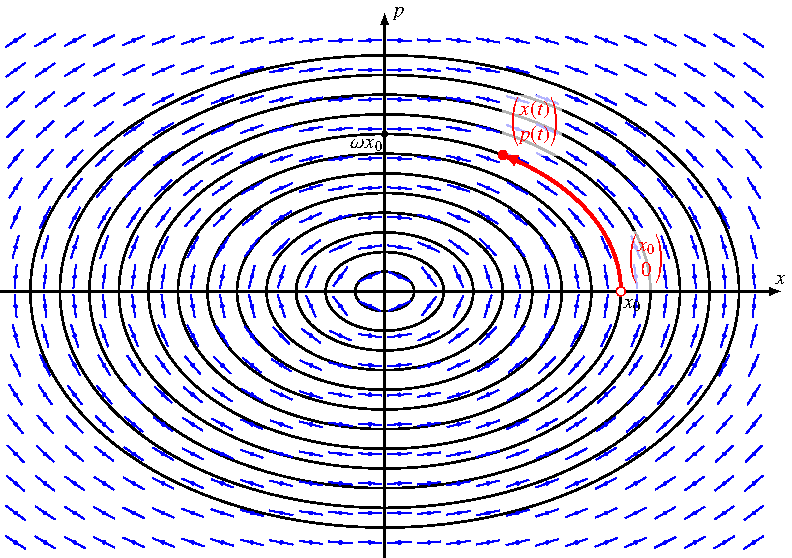
\includegraphics{chapters/60-gruppen/images/phasenraum.pdf}
\caption{Die Lösungen der
Differentialgleichung~\eqref{chapter:gruppen:eqn:phasenraumdgl}
im Phasenraum sind Ellipsen mit Halbachsenverhältnis $\omega^{-1}$.
\label{chapter:gruppen:fig:phasenraum}}
\end{figure}
Eine Masse $m$ verbunden mit einer Feder mit der Federkonstanten $K$
schwingt um die Ruhelage $x=0$ entsprechend der Differentialgleichung
\[
m\frac{d^2}{dt^2} x(t) =  -Kx(t).
\]
Die Kreisfrequenz der Schwingung ist
\[
\omega = \sqrt{\frac{K}{m}}.
\]
Das System kann als zweidimensionales System im Phasenraum mit den 
Koordinaten $x_1=x$ und $x_2=p=m\dot{x}$ beschrieben werden.
Die zweidimensionale Differentialgleichung ist
\begin{equation}
\left.
\begin{aligned}
\dot{x}(t) &= \frac{1}{m}p(t)\\
\dot{p}(t) &= -Kx(t) 
\end{aligned}
\quad
\right\}
\qquad\Rightarrow\qquad
\frac{d}{dt}
\begin{pmatrix}x(t)\\p(t)\end{pmatrix}
=
\begin{pmatrix}
0&\frac{1}{m}\\
-K&0
\end{pmatrix}
\begin{pmatrix}x(t)\\p(t)\end{pmatrix}.
\label{chapter:gruppen:eqn:phasenraumdgl}
\end{equation}
Die Lösung der Differentialgleichung für die Anfangsbedingung $x(0)=1$ und
$p(0)=0$ ist
\[
x(t)
=
\cos \omega t
\qquad\Rightarrow\qquad
p(t)
=
-\omega \sin\omega t,
\]
die Lösung zur Anfangsbedingung $x(0)=0$ und $p(0)=1$ ist
\[
x(t) = \frac{1}{\omega} \sin\omega t,
\qquad
p(t) = \cos \omega t.
\]
In Matrixform kann man die allgemeine Lösung zur Anfangsbedingun $x(0)=x_0$
und $p(0)=p_0$
\begin{equation}
\begin{pmatrix}
x(t)\\
p(t)
\end{pmatrix}
=
\underbrace{
\begin{pmatrix}
 \cos \omega t & \frac{1}{\omega} \sin\omega t \\
-\omega \sin\omega t & \cos\omega t
\end{pmatrix}
}_{\displaystyle =\Phi_t}
\begin{pmatrix}x_0\\p_0\end{pmatrix}
\label{buch:gruppen:eqn:phi}
\end{equation}
schreiben.
Die Matrizen $\Phi_t$ bilden eine Einparameter-Untergruppe von
$\operatorname{GL}_n(\mathbb{R})$, da
\begin{align*}
\Phi_s\Phi_t
&=
\begin{pmatrix}
 \cos\omega s & \frac{1}{\omega} \sin\omega s \\
-\omega \sin\omega s & \cos\omega s
\end{pmatrix}
\begin{pmatrix}
 \cos\omega t & \frac{1}{\omega} \sin\omega t \\
-\omega \sin\omega t & \cos\omega t
\end{pmatrix}
\\
&=
\begin{pmatrix}
\cos\omega s \cos\omega t - \sin\omega s \sin\omega t 
& \frac{1}{\omega} ( \cos\omega s \sin\omega t + \sin\omega s \cos \omega t)
\\
-\omega (\sin\omega s \cos\omega t + \cos\omega s \sin\omega t )
& \cos\omega s \cos\omega t -\sin\omega s \sin\omega t 
\end{pmatrix}
\\
&=
\begin{pmatrix}
 \cos\omega(s+t) & \frac{1}{\omega}\sin\omega(s+t) \\
-\omega \sin\omega(s+t) & \cos\omega(s+t)
\end{pmatrix}
=
\Phi_{s+t}
\end{align*}
gilt.
Die Lösungen der 
Differentialgleichung~\eqref{chapter:gruppen:eqn:phasenraumdgl}
sind in Abbildung~\ref{chapter:gruppen:fig:phasenraum}
Die Matrizen $\Phi_t$ beschreiben eine kontinuierliche Symmetrie
des Differentialgleichungssystems, welches den harmonischen Oszillator
beschreibt.

\subsubsection{Fluss einer Differentialgleichung}
Die Abbildungen $\Phi_t$ von \eqref{buch:gruppen:eqn:phi} sind jeweils
Matrizen in $\operatorname{GL}_n(\mathbb{R})$.
Der Grund dafür ist, dass die
Differentialgleichung~\eqref{chapter:gruppen:eqn:phasenraumdgl}
linear ist.
Dies hat zur Folge, dass für zwei Anfangsbedingungen $x_1,x_2\in\mathbb{R}^2$
die Lösung für Linearkombinationen $\lambda x_1+\mu x_2$ durch
Linearkombination der Lösungen erhalten werden kann, also
aus der Formel
\[
\Phi_t (\lambda x_1 + \mu x_2) = \lambda \Phi_t x_1 + \mu \Phi_t x_2.
\]
Dies zeigt, dass $\Phi_t$ für jedes $t$ eine lineare Abbildung sein muss.

Für eine beliebige Differentialgleichung kann man immer noch eine Abbildung
$\Phi$ konstruieren, die aber nicht mehr linear ist.
Sei dazu die Differentialgleichung erster Ordnung
\begin{equation}
\frac{dx}{dt}
=
f(t,x)
\qquad\text{mit}\qquad
f\colon \mathbb{R}\times\mathbb{R}^n \to \mathbb{R}^n
\label{buch:gruppen:eqn:dgl}
\end{equation}
gegeben.
Für jeden Anfangswert $x_0\in\mathbb{R}^n$ kann man mindestens für eine
gewisse Zeit $t <\varepsilon$ eine Lösung $x(t,x_0)$ finden mit $x(t,x_0)=x_0$.
Aus der Theorie der gewöhnlichen Differentialgleichungen ist auch
bekannt, dass $x(t,x_0)$ mindestens in der Nähe von $x_0$ differenzierbar von
$x_0$ abhängt.
Dies erlaubt eine Abbildung
\[
\Phi\colon \mathbb{R}\times \mathbb{R}^n \to \mathbb{R}^n
:
(t,x_0) \mapsto \Phi_t(x_0) = x(t,x_0)
\]
zu definieren, die sowohl von $t$ als auch von $x_0$ differenzierbar
abhängt.
Aus der Definition folgt unmittelbar, dass $\Phi_0(x_0)=x_0$ ist, dass
also $\Phi_0$ die identische Abbildung von $\mathbb{R}^n$ ist.

Aus der Definition lässt sich auch ableiten, dass
$\Phi_{s+t}=\Phi_s\circ\Phi_t$ gilt.
$\Phi_t(x_0)=x(t,x_0)$ ist der Endpunkt der Bahn, die bei $x_0$ beginnt
und sich während der Zeit $t$ entwickelt.
$\Phi_s(x(t,x_0))$ ist dann der Endpunkt der Bahn, die bei $x(t,x_0)$ 
beginnt und sich während der Zeit $s$ entwickelt.
Somit ist $\Phi_s\circ \Phi_t(x_0)$ der Endpunkt der Bahn, die bei
$x_0$ beginnt und sich über die Zeit $s+t$ entwickelt.
In Formeln bedeutet dies
\[
\Phi_{s+t} = \Phi_s\circ \Phi_t.
\]
Die Abbildung $t\mapsto \Phi_t$ ist also wieder ein Homomorphismus
von der additiven Gruppe $\mathbb{R}$ in eine Gruppe von differenzierbaren
Abbildungen $\mathbb{R}^n\to\mathbb{R}^n$.

\begin{definition}
Die Abbildung
\[
\Phi\colon \mathbb{R}\times\mathbb{R}^n\to\mathbb{R}^n
:
(t,x_0) \mapsto \Phi_t(x_0) = x(t,x_0)
\]
heisst der {\em Fluss} der Differentialgleichung
\eqref{buch:gruppen:eqn:dgl},
wenn für jedes $x_0\in\mathbb{R}^n$ die Kurve $t\mapsto \Phi_t(x_0)$
eine Lösung der Differentialgleichung ist mit Anfangsbedingung $x_0$.
\end{definition}

Die Abbildung $\Phi_t$ von \eqref{buch:gruppen:eqn:phi} ist also
der Fluss der Differentialgleichung des harmonischen Oszillators.

\subsection{Mannigfaltigkeiten
\label{buch:subsection:mannigfaltigkeit}}
Eine Differentialgleichung der Form~\eqref{buch:gruppen:eqn:dgl}
stellt einen Zusammenhang her zwischen einem Punkt $x$ und der
Tangentialrichtung einer Bahnkurve $f(t,x)$.
Die Ableitung liefert die lineare Näherung der Bahkurve
\[
x(t_0+h) = x(t_0) + h f(t_0,x_0) + o(h)
\]
für $h$ in einer kleinen Umgebung von $0$.
Das funktioniert auch, weil $f(t_0,x_0)$ selbst ein Vektor von
$\mathbb{R}^n$ ist, in dem die Bahnkurve verläuft.

Diese Idee funktioniert nicht mehr zum Beispiel für eine
Differentialgleichung auf einer Kugeloberfläche, weil alle Punkte
$x(t_0)+hf(t_0,x_0)$ für alle $h\ne 0$ nicht mehr auf der Kugeloberfläche
liegen.
Physikalisch äussert sich das ein einer zusätzlichen Kraft, die nötig
ist, die Bahn auf der Kugeloberfläche zu halten.
Diese Kraft stellt zum Beispiel sicher, dass die Vektoren $f(t,x)$ für
Punkte $x$ auf der Kugeloberfläche immer tangential an die Kugel sind.
Trotzdem ist der Tangentialvektor oder der Geschwindigkeitsvektor 
nicht mehr ein Objekt, welches als Teil der Kugeloberfläche definiert
werden kann, er kann nur definiert werden, wenn man sich die Kugel als
in einen höherdimensionalen Raum eingebettet vorstellen kann.

Um die Idee der Differentialgleichung auf einer beliebigen Fläche
konsistent zu machen ist daher notwendig, die Idee einer Tagentialrichtung
auf eine Art zu definieren, die nicht von der Einbettung der Fläche
in den $n$-dimensionalen Raum abhängig ist.
Das in diesem Abschnitt entwickelte Konzept der {\em Mannigfaltigkeit}
löst dieses Problem.

\subsubsection{Karten}
Die Navigation auf der Erdoberfläche verwendet das Koordinatensystem
der geographischen Länge und Breite.
Dieses Koordinatensystem funktioniert gut, solange man sich nicht an
den geographischen Polen befindet, denn deren Koordinaten sind
nicht mehr eindeutig.
Alle Punkte mit geographischer Breite $90^\circ$ und beliebiger 
geographischer Länge beschreiben den Nordpol.
Auch die Ableitung funktioniert dort nicht mehr.
Bewegt man sich mit konstanter Geschwindigkeit über den Nordpol,
springt die Ableitung der geographischen Breite von einem positiven
Wert auf einen negativen Wert, sie kann also nicht differenzierbar sein.
Diese Einschränkungen sind in der Praxis nur ein geringes Problem dar,
da die meisten Reisen nicht über die Pole erfolgen.

Der Polarforscher, der in unmittelbarer Umgebung des Poles arbeitet,
kann das Problem lösen, indem er eine lokale Karte für das Gebiet
um den Pol erstellt.
Dafür kann er beliebige Koordinaten verwenden, zum Beispiel auch
ein kartesisches Koordinatensystem, er muss nur eine Methode haben,
wie er seine Koordinaten wieder auf geographische Länge und Breite
umrechnen will.
Und wenn er über Geschwindigkeiten kommunizieren will, dann muss
er auch Ableitungen von Kurven in seinem kartesischen Koordinatensystem
umrechnen können auf die Kugelkoordinaten.
Dazu muss seine Umrechnungsformel von kartesischen Koordinaten
auf Kugelkoordinaten differenzierbar sein.

Diese Idee wird durch das Konzept der Mannigfaltigkeit verallgemeinert.
Eine $n$-dimensionale {\em Mannigfaltigkeit} ist eine Menge $M$ von Punkten,
die lokal, also in der Umgebung eines Punktes, mit möglicherweise mehreren
verschiedenen Koordinatensystemen versehen werden kann.
Ein Koordinatensystem ist eine umkehrbare Abbildung einer offenen Teilmenge
$U\subset M$ in den Raum $\mathbb{R}^n$.
Die Komponenten dieser Abbildung heissen die {\em Koordinaten}.

\begin{figure}
\centering
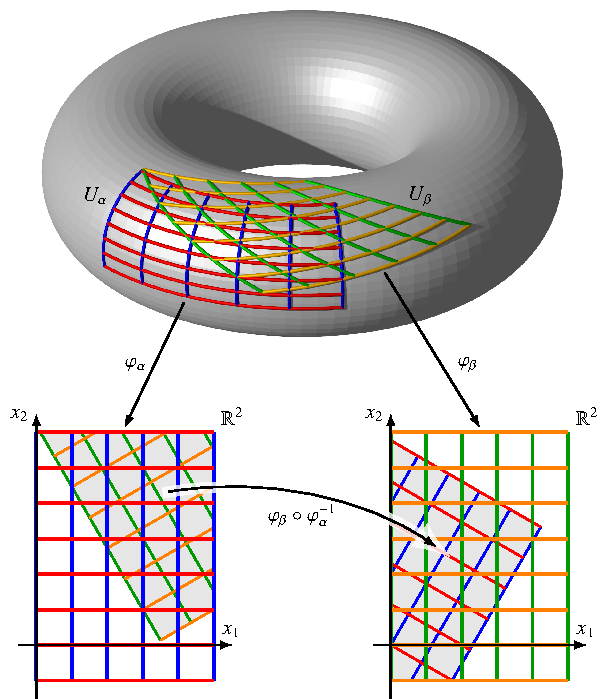
\includegraphics{chapters/60-gruppen/images/karten.pdf}
\caption{Karten
$\varphi_\alpha\colon U_\alpha\to \mathbb{R}^2$
und
$\varphi_\beta\colon U_\beta\to \mathbb{R}^2$
auf einem Torus.
Auf dem Überschneidungsgebiet $\varphi_\alpha^{-1}(U_\alpha\cap U_\beta)$
ist der Kartenwechsel $\varphi_\beta\circ\varphi_\alpha^{-1}$ wohldefiniert
und muss differnzierbar sein, wenn eine differenzierbare Mannigfaltigkeit
entstehen soll.
\label{buch:gruppen:fig:karten}}
\end{figure}

\begin{definition}
Eine Karte auf $M$ ist eine umkehrbare Abbildung
$\varphi\colon U\to \mathbb{R}^n$ (siehe auch
Abbildung~\ref{buch:gruppen:fig:karten}).
Ein differenzierbarer Atlas ist eine Familie von Karten $\varphi_\alpha$
derart, dass die Definitionsgebiete $U_\alpha$ die ganze Menge $M$
überdecken, und dass die Kartenwechsel Abbildungen
\[
\varphi_{\beta\alpha}=\varphi_\beta\circ\varphi_\alpha^{-1}
\colon
\varphi_\alpha(U_\alpha\cap U_\beta)
\to
\varphi_\beta(U_\alpha\cap U_\beta)
\]
als Abbildung von offenen Teilmengen von $\mathbb{R}^n$ differenzierbar
ist.
Eine {$n$-dimensionale differenzierbare Mannigfaltigkeit} ist eine
Menge $M$ mit einem differenzierbaren Atlas.
\end{definition}

Karten und Atlanten regeln also nur, wie sich verschiedene lokale
Koordinatensysteme ineinander umrechnen lassen.

\begin{beispiel}
$M=\mathbb{R}^n$ ist eine differenzierbare Mannigfaltigkeit denn 
die identische Abbildung $M\to \mathbb{R}^n$ ist eine Karte und ein
Atlas von $M$.
\end{beispiel}

\begin{beispiel}
\begin{figure}
\centering
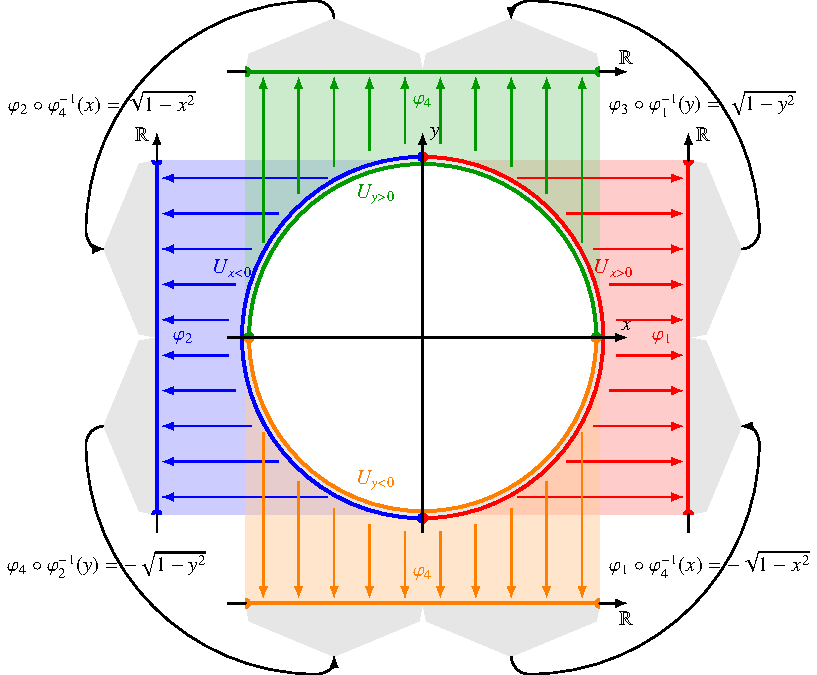
\includegraphics{chapters/60-gruppen/images/kartenkreis.pdf}
\caption{Karten für die Kreislinie $S^1\subset\mathbb{R}^2$.
\label{buch:gruppen:fig:kartenkreis}}
\end{figure}
Die Kreislinie in in der Ebene ist eine $1$-dimensionale Mannigfaltigkeit.
Natürlich kann sie nicht mit einer einzigen Karte beschrieben werden,
da es keine umkehrbaren Abbildungen zwischen $\mathbb{R}$ und der Kreislinie
gibt.
Man kann aber die folgenden vier Karten verwenden:
\begin{align*}
\varphi_1&\colon U_{x>0}\{(x,y)\;|\;x^2+y^2=1\wedge x>0\} \to
:
(x,y) \mapsto y\\
\varphi_2&\colon U_{x<0}\{(x,y)\;|\;x^2+y^2=1\wedge x<0\} \to
:
(x,y) \mapsto y\\
\varphi_3&\colon U_{y>0}\{(x,y)\;|\;x^2+y^2=1\wedge y>0\} \to
:
(x,y) \mapsto x\\
\varphi_4&\colon U_{y<0}\{(x,y)\;|\;x^2+y^2=1\wedge y<0\} \to
:
(x,y) \mapsto x
\end{align*}
Die Werte der Kartenabbildungen sind genau die $x$- und $y$-Koordinaten
auf der in den Raum $\mathbb{R}^2$ eingebetteten Kreislinie.

Für $\varphi_1$ und $\varphi_2$ sind die Definitionsgebiete disjunkt,
hier gibt es also keine Notwendigkeit, Koordinatenumrechnungen vornehmen
zu können.
Dasselbe gilt für $\varphi_3$ und $\varphi_4$.

Die nichtleeren Schnittmengen der verschiedenen Kartengebiete beschreiben
jeweils die Punkte der Kreislinie in einem Quadranten.
Die Umrechnung zwischen den Koordinaten erfolgt je nach Quadrant durch
\[
x\mapsto y=\pm\sqrt{1-x^2\mathstrut}
\qquad\text{oder}\qquad
y\mapsto x=\pm\sqrt{1-y^2\mathstrut},
\]
diese Abbildungen sind im offenen Intervall $(-1,1)$ differenzierbar,
Schwierigkeiten mit der Ableitungen ergeben sich nur an den Stellen
$x=\pm1$ und $y=\pm 1$, die in einem Überschneidungsgebiet von Karten
nicht vorkommen können.
Somit bilden die vier Karten einen differenzierbaren Atlas für
die Kreislinie (Abbildung~\ref{buch:gruppen:fig:kartenkreis}).
\end{beispiel}

\begin{beispiel}
Ganz analog zum vorangegangenen Beispiel über die Kreisline lässt sich
für eine $n$-di\-men\-sio\-nale Sphäre
\[
S^n = \{ (x_1,\dots,x_{n+1})\;|\; x_0^2+\dots+x_n^2=1\}
\]
immer ein Atlas aus $2^{n+1}$ Karten mit den Koordinatenabbildungen
\[
\varphi_{i,\pm}
\colon
U_{i,\pm}
=
\{p\in S^n\;|\; \pm x_i >0\}
\to
\mathbb{R}^n
:
p\mapsto (x_1,\dots,\hat{x}_i,\dots,x_{n+1})
\]
konstruieren, der $S^n$ zu einer $n$-dimensionalen Mannigfaltigkeit macht.
\end{beispiel}

\subsubsection{Tangentialraum}
Mit Hilfe einer Karte $\varphi_\alpha\colon U_\alpha\to\mathbb{R}^n$
kann das Geschehen in einer Mannigfaltigkeit in den vertrauten 
$n$-dimensionalen Raum $\mathbb{B}^n$ transportiert werden. 
Eine Kurve $\gamma\colon \mathbb{R}\to M$, die so parametrisiert sein
soll, dass $\gamma(t)\in U_\alpha$ für $t$ in einer Umgebung $I$ von $0$ ist,
wird von der Karte in eine Kurve
$\gamma_\alpha=\varphi_\alpha\circ\gamma\colon I\to \mathbb{R}^n$ 
abgebildet,
deren Tangentialvektor wieder ein Vektor in $\mathbb{R}^n$ ist.

Eine zweite Karte $\varphi_\beta$ führt auf eine andere Kurve
mit der Parametrisierung
$\gamma_\beta=\varphi_\beta\circ\gamma\colon I \to \mathbb{R}^n$ 
und einem anderen Tangentialvektor.
Die beiden Tangentialvektoren können aber mit der Ableitung der
Koordinatenwechsel-Abbildung
$\varphi_{\beta\alpha}=\varphi_\beta\circ\varphi_\alpha^{-1}\colon
\varphi_\alpha(U_\alpha\cap U_\beta)\to \mathbb{R}^n$
ineinander umgerechnet werden.
Aus
\[
\gamma_\beta
=
\varphi_\beta\circ \gamma
=
(
\varphi_\beta
\circ
\varphi_\alpha^{-1}
)
\circ
\varphi_\alpha\circ\gamma
=
\varphi_{\beta\alpha}
\circ
\varphi_\alpha\circ\gamma
=
\varphi_{\beta\alpha}\circ\gamma_\alpha
\]
folgt durch Ableitung nach dem Kurvenparameter $t$, dass
\[
\frac{d}{dt}\gamma_\beta(t)
=
D\varphi_{\beta\alpha} \frac{d}{dt}\gamma_\alpha(t).
\]
Die Ableitung $D\varphi_{\beta\alpha}$ von $\varphi_{\beta\alpha}$ 
an der Stelle $\gamma_\alpha(t)$ berechnet also aus dem Tangentialvektor
einer Kurve in der Karte $\varphi_\alpha$ den Tangentialvektor der
Kurve in der Karte $\varphi_\beta$.

Die Forderung nach Differenzierbarkeit der Kartenwechselabbildungen
$\varphi_{\beta\alpha}$ stellt also nur sicher, dass die Beschreibung
eines Systemes mit Differentialgleichungen in verschiedenen
Koordinatensystemen auf die gleichen Lösungskurven in der
Mannigfaltigkeit führt.
Insbesondere ist die Verwendung von Karten ist also nur ein Werkzeug,
mit dem die Unmöglichkeit einer globalen Besschreibung einer
Mannigfaltigkeit $M$ mit einem einzigen globalen Koordinatensystem
ohne Singularitäten umgangen werden kann.

\subsection{Der Satz von Noether
\label{buch:subsection:noether}}








%
% lie-gruppen.tex -- Lie-Gruppebn
%
% (c) 2020 Prof Dr Andreas Müller, Hochschule Rapperswil
%
\section{Lie-Gruppen
\label{buch:section:lie-gruppen}}
\rhead{Lie-Gruppen}
Die in bisherigen Beispielen untersuchten Matrizengruppen zeichnen sich
durch zusätzliche Eigenschaften aus.
Die Gruppe
\[
\operatorname{GL}_n(\mathbb{R}) 
=
\{ A \in M_n(\mathbb{R})\;|\; \det A \ne 0\}
\]
besteht aus den Matrizen, deren Determinante nicht $0$ ist.
Da die Menge der Matrizen mit $\det A=0$ eine abgeschlossene Menge
in $M_n(\mathbb{R}) \simeq \mathbb{R}^{n^2}$ ist, ist
$\operatorname{GL}_n(\mathbb{R})$ eine offene Teilmenge in $\mathbb{R}^{n^2}$,
sie besitzt also automatisch die Struktur einer $n^2$-Mannigfaltigkeit.
Dies gilt jedoch auch für alle anderen Matrizengruppen, die in diesem
Abschnitt genauer untersucht werden sollen.

\subsection{Mannigfaltigkeitsstruktur der Matrizengruppen
\label{buch:subsection:mannigfaltigkeitsstruktur-der-matrizengruppen}}
Eine Matrizengruppe wird automatsich zu einer Mannigfaltigkeit,
wenn es gelingt, eine Karte für eine Umgebung des neutralen Elements
zu finden.
Dazu muss gezeigt werden, dass sich aus einer solchen Karte für jedes
andere Gruppenelement eine Karte für eine Umgebung ableiten lässt.
Sei also $\varphi_e\colon U_e\mathbb{R}^N$ eine Karte für die Umgebung
$U_e\subset G$ von $e\in G$.
Für $g\in G$ ist dann die Abbildung
\[
\varphi_g
\colon
U_g
=
gU_e
\to
\mathbb{R}
:
h\mapsto \varphi_e(g^{-1}h)
\]
eine Karte für die Umgebung $U_g$ des Gruppenelementes $g$.
schreibt man $l_{g}$ für  die Abbildung $h\mapsto gh$, dann
kann man die Kartenabbildung auch $\varphi_g = \varphi_e\circ l_{g^{-1}}$
schreiben.

\subsubsection{Kartenwechsel}
Die Kartenwechsel-Abbildungen für zwei Karten $\varphi_{g_1}$
und $\varphi_{g_2}$ ist die Abbildung
\[
\varphi_{g_1,g_2}
=
\varphi_{g_1}\circ \varphi_{g_2}^{-1}
=
\varphi_e\circ l_{g_1^{-1}} \circ (\varphi_e\circ l_{g_2^{-1}})^{-1}
=
\varphi_e\circ l_{g_1^{-1}} \circ l_{g_2^{-1}}^{-1} \varphi_e^{-1}
=
\varphi_e\circ l_{g_1^{-1}} \circ l_{g_2}\varphi_e^{-1}
=
\varphi_e\circ l_{g_1^{-1}g_2}\varphi_e^{-1}
\]
mit der Ableitung
\[
D\varphi_e\circ Dl_{g_1^{-1}g_2} D\varphi_e^{-1}
=
D\varphi_e\circ Dl_{g_1^{-1}g_2} (D\varphi_e)^{-1}.
\]
Die Abbildung $l_{g_1^{-1}g_2}$ ist aber nur die Multiplikation mit
einer Matrix, also eine lineare Abbildung, so dass der Kartenwechsel
nichts anderes ist als die Darstellung der Matrix der Linksmultiplikation
$l_{g_1^{-1}g_2}$ im Koordinatensystem der Karte $U_e$ ist.
Differenzierbarkeit der Kartenwechsel ist damit sichergestellt,
die Matrizengruppen sind automatisch differenzierbare Mannigfaltigkeiten.

Die Konstruktion aller Karten aus einer einzigen Karte für eine
Umgebung des neutralen Elements zeigt auch, dass es für die Matrizengruppen
reicht, wenn man die Elemente in einer Umgebung des neutralen
Elementes parametrisieren kann.
Dies ist jedoch nicht nur für die Matrizengruppen möglich.
Wenn eine Gruppe gleichzeitig eine differenzierbare Mannigfaltigkeit
ist, dann können Karten über die ganze Gruppe transportiert werden,
wenn die Multiplikation mit Gruppenelementen eine differenzierbare
Abbildung ist.
Solche Gruppen heissen auch Lie-Gruppen gemäss der folgenden Definition.

\begin{definition}
\index{Lie-Gruppe}%
Eine {\em Lie-Gruppe} ist eine Gruppe, die gleichzeitig eine differenzierbare
Mannigfaltigkeit ist derart, dass die Abbildungen
\begin{align*}
G\times G \to G &: (g_1,g_2)\mapsto g_1g_2
\\
G\to G &: g \mapsto g^{-1}
\end{align*}
differenzierbare Abbildungen zwischen Mannigfaltigkeiten sind.
\end{definition}

Die Abstraktheit dieser Definition täuscht etwas über die 
Tatsache hinweg, dass sich mit Hilfe der Darstellungstheorie
jede beliebige Lie-Gruppe als Untermannigfaltigkeit einer 
Matrizengruppe verstehen lässt.
Das Studium der Matrizengruppen erlaubt uns daher ohne grosse
Einschränkungen ein Verständnis für die Theorie der Lie-Gruppen
zu entwickeln.

\subsubsection{Tangentialvektoren und die Exponentialabbildung}
Die Matrizengruppen sind alle in der
$n^2$-dimensionalen Mannigfaltigkeit $\operatorname{GL}_n(\mathbb{R})$
enthalten.
Diffferenzierbare Kurven $\gamma(t)$ in $\operatorname{GL}_n(\mathbb{R})$
haben daher in jedem Punkt Tangentialvektoren, die als Matrizen in
$M_n(\mathbb{R})$ betrachtet werden können.
Wenn $\gamma(t)$ die Matrixelemente $\gamma_{ij}(t)$ hat, dann ist der
Tangentialvektor im Punkt $\gamma(t)$ durch
\[
\frac{d}{dt}
\gamma(t)
=
\begin{pmatrix}
\dot{\gamma}_{11}(t)&\dots &\dot{\gamma}_{1n}(t)\\
\vdots              &\ddots&\vdots              \\
\dot{\gamma}_{n1}(t)&\dots &\dot{\gamma}_{nn}(t)
\end{pmatrix}
\]
gegeben.

Im Allgemeinen kann man Tangentialvektoren in verschiedenen Punkten
einer Mannigfaltigkeit nicht miteinander vergleichen.
Die Multiplikation $l_g$, die den Punkt $e$ in den Punkt $g$ verschiebt,
transportiert auch die Tangentialvektoren im Punkt $e$ in 
Tangentialvektoren im Punkt $g$.

\begin{aufgabe}
Gibt es eine Kurve $\gamma(t)\in\mathbb{GL}_n(\mathbb{R})$ mit
$\gamma(0)=e$ derart, dass der Tangentialvektor im Punkt $\gamma(t)$
für $t>0$ derselbe ist wie der Tangentialvektor im Punkt $e$, transportiert
durch Matrixmultiplikation mit $\gamma(t)$?
\end{aufgabe}

Eine solche Kurve muss die Differentialgleichung
\begin{equation}
\frac{d}{dt}\gamma(t)
=
\gamma(t)\cdot A
\label{buch:gruppen:eqn:expdgl}
\end{equation}
erfüllen, wobei $A\in M_n(\mathbb{R})$ der gegebene Tangentialvektor
in $e=I$ ist.

Die Matrixexponentialfunktion
\[
e^{At}
=
1+At+\frac{A^2t^2}{2!}+\frac{A^3t^3}{3!}+\frac{A^4t^4}{4!}+\dots
\]
liefert eine Einparametergruppe
$\mathbb{R}\to \operatorname{GL}_n(\mathbb{R})$ mit der Ableitung
\[
\frac{d}{dt} e^{At}
=
\lim_{h\to 0} \frac{e^{A(t+h)}-e^{At}}{h}
=
\lim_{h\to 0} e^{At}\frac{e^{Ah}-I}{h}
=
e^{At} A.
\]
Sie ist also Lösung der Differentialgleichung~\eqref{buch:gruppen:eqn:expdgl}.

\subsection{Drehungen in der Ebene
\label{buch:gruppen:drehungen2d}}
Die Drehungen der Ebene sind die orientierungserhaltenden Symmetrien
des Einheitskreises, der in Abbildung~\ref{buch:gruppen:fig:kartenkreis}
als Mannigfaltigkeit erkannt wurde.
Sie bilden eine Lie-Gruppe, die auf verschiedene Arten als Matrix
beschrieben werden kann.

\subsubsection{Die Untergruppe
$\operatorname{SO}(2)\subset \operatorname{GL}_2(\mathbb{R})$}
Drehungen der Ebene können in einer orthonormierten Basis durch
Matrizen der Form
\[
D_{\alpha}
=
\begin{pmatrix}
\cos\alpha&-\sin\alpha\\
\sin\alpha& \cos\alpha
\end{pmatrix}
\]
dargestellt werden.
Wir bezeichnen die Menge der Drehmatrizen in der Ebene mit
$\operatorname{SO}(2)\subset\operatorname{GL}_2(\mathbb{R})$.
Die Abbildung
\[
D_{\bullet}
\colon
\mathbb{R}\to \operatorname{SO}(2)
:
\alpha \mapsto D_{\alpha}
\]
hat die Eigenschaften
\begin{align*}
D_{\alpha+\beta}&= D_{\alpha}D_{\beta}
\\
D_0&=I
\\
D_{2k\pi}&=I\qquad \forall k\in\mathbb{Z}.
\end{align*}
Daraus folgt zum Beispiel, dass $D_{\bullet}$ eine $2\pi$-periodische
Funktion ist.
$D_{\bullet}$ bildet die Menge der Winkel $[0,2\pi)$ bijektiv auf
die Menge der Drehmatrizen in der Ebene ab.

Für jedes Intervall $(a,b)\subset\mathbb{R}$ mit Länge
$b-a < 2\pi$ ist die Abbildung $\alpha\mapsto D_{\alpha}$ umkehrbar,
die Umkehrung kann als Karte verwendet werden.
Zwei verschiedene Karten $\alpha_1\colon U_1\to\mathbb{R}$ und
$\alpha_2\colon U_2\to\mathbb{R}$ bilden die Elemente $g\in U_1\cap U_2$
in Winkel $\alpha_1(g)$ und $\alpha_2(g)$ ab, für die 
$D_{\alpha_1(g)}=D_{\alpha_2(g)}$ gilt.
Dies ist gleichbedeutend damit, dass $\alpha_1(g)=\alpha_2(g)+2\pi k$
mit $k\in \mathbb{Z}$.
In einem Intervall in $U_1\cap U_2$ muss $k$ konstant sein.
Die Kartenwechselabblidung ist also nur die Addition eines Vielfachen
von $2\pi$, mit der identischen Abbildung als Ableitung.
Diese Karten führen also auf besonders einfache Kartenwechselabbildungen.

\subsubsection{Die Untergruppe $S^1\subset\mathbb{C}$}
Ein alternatives Bild für die Drehungen der Ebene kann man in der komplexen
Ebene $\mathbb{C}$ erhalten.
Die Multiplikation mit der komplexen Zahl $e^{i\alpha}$ beschreibt eine
Drehung der komplexen Ebene um den Winkel $\alpha$.
Die Zahlen der Form $e^{i\alpha}$ haben den Betrag $1$ und die Abbildung
\[
f\colon \mathbb{R}\to \mathbb{C}:\alpha \mapsto e^{i\alpha}
\]
hat die Eigenschaften
\begin{align*}
f(\alpha+\beta) &= f(\alpha)f(\beta)
\\
f(0)&=1
\\
f(2\pi k)&=1\qquad\forall k\in\mathbb{Z},
\end{align*}
die zu den Eigenschaften der Abbildung $\alpha\mapsto D_{\alpha}$ 
analog sind.

Jede komplexe Zahl $z$ vom Betrag $1$ kann geschrieben werden in der Form
$z=e^{i\alpha}$, die Abbildung $f$ ist also eine Parametrisierung des
Einheitskreises in der Ebene.
Wir bezeichen $S^1=\{z\in\mathbb{C}\;|\; |z|=1\}$ die komplexen Zahlen vom
Betrag $1$.
$S^1$ ist eine Gruppe bezüglich der Multiplikation, da für jede Zahl
$z,w\in S^1$ gilt
$|z^{-1}|=1$ und $|zw|=1$ und damit $z^{-1}\in S^1$ und $zw\in S^1$.

Zu einer komplexen Zahl $z\in S^1$ gibt es einen bis auf Vielfache
von $2\pi$ eindeutigen Winkel $\alpha(z)$ derart, dass $e^{i\alpha(z)}=z$.
Damit kann man jetzt die Abbildung
\[
\varphi
\colon
S^1\to \operatorname{SO}(2)
:
z\mapsto  D_{\alpha(z)}
\]
konstruieren.
Da $D_{\alpha}$ $2\pi$-periodisch ist, geben um Vielfache
von $2\pi$ verschiedene Wahlen von $\alpha(z)$ die gleiche
Matrix $D_{\alpha(z)}$, die Abbildung $\varphi$ ist daher
wohldefiniert.
$\varphi$ erfüllt ausserdem die Bedingungen
\begin{align*}
\varphi(z_1z_2)
&=
D_{\alpha(z_1z_2)}
=
D_{\alpha(z_1)+\alpha(z_2)}
=
D_{\alpha(z_1)}D_{\alpha(z_2)}
=
\varphi(z_1)\varphi(z_2)
\\
\varphi(1)
&=
D_{\alpha(1)}
=
D_0
=
I
\end{align*}
Die Abbildung $\varphi$ ist ein Homomorphismus der Gruppe $S^1$
in die Gruppe $\operatorname{SO}(2)$.
Die Menge der Drehmatrizen in der Ebene kann also mit dem Einheitskreis
in der komplexen Ebene identifiziert werden.

\subsubsection{Tangentialvektoren von $\operatorname{SO}(2)$}
Da die Gruppe $\operatorname{SO}(2)$ eine eindimensionale Gruppe
ist, kann jede Kurve $\gamma(t)$ durch den Drehwinkel $\alpha(t)$
mit $\gamma(t) = D_{\alpha(t)}$ beschrieben werden.
Die Ableitung in $M_2(\mathbb{R})$ ist
\begin{align*}
\frac{d}{dt} \gamma(t)
&=
\frac{d}{d\alpha}
\begin{pmatrix}
\cos\alpha(t) & - \sin\alpha(t)\\
\sin\alpha(t) &   \cos\alpha(t)
\end{pmatrix}
\cdot
\frac{d\alpha}{dt}
\\
&=
\begin{pmatrix}
-\sin\alpha(t)&-\cos\alpha(t)\\
 \cos\alpha(t)&-\sin\alpha(t)
\end{pmatrix}
\cdot
\dot{\alpha}(t)
\\
&=
\begin{pmatrix}
\cos\alpha(t) & - \sin\alpha(t)\\
\sin\alpha(t) &   \cos\alpha(t)
\end{pmatrix}
\begin{pmatrix}
0&-1\\
1&0
\end{pmatrix}
\cdot
\dot{\alpha}(t)
=
D_{\alpha(t)}J\cdot\dot{\alpha}(t).
\end{align*}
Alle Tangentialvektoren von $\operatorname{SO}(2)$ im Punkt $D_\alpha$
entstehen aus $J$ durch Drehung mit der Matrix $D_\alpha$ und Skalierung
mit $\dot{\alpha}(t)$.

%
% Isometrien von R^n
%
\subsection{Isometrien von $\mathbb{R}^n$
\label{buch:gruppen:isometrien}}

\subsubsection{Skalarprodukt}
Lineare Abbildungen des Raumes $\mathbb{R}^n$ können durch
$n\times n$-Matrizen beschrieben werden.
Die Matrizen, die das Standardskalarprodukt $\mathbb{R}^n$ erhalten,
bilden eine Gruppe, die in diesem Abschnitt genauer untersucht werden soll.
Eine Matrix $A\in M_{n}(\mathbb{R})$ ändert das Skalarprodukt, wenn
für jedes beliebige Paar $x,y$ von Vektoren gilt
$\langle Ax,Ay\rangle = \langle x,y\rangle$.
Das Standardskalarprodukt kann mit dem Matrixprodukt ausgedrückt werden:
\[
\langle Ax,Ay\rangle
=
(Ax)^tAy
=
x^tA^tAy
=
x^ty
=
\langle x,y\rangle
\]
für jedes Paar von Vektoren $x,y\in\mathbb{R}$.

Mit dem Skalarprodukt kann man auch die Matrixelemente einer Matrix
einer Abbildung $f$ in der Standardbasis bestimmen.
Das Skalarprodukt $\langle e_i, v\rangle$ ist die Länge der Projektion
des Vektors $v$ auf die Richtung $e_i$.
Die Komponenten von $Ae_j$ sind daher $a_{ij}=\langle e_i,f(e_j)\rangle$.
Die Matrix $A$ der Abbildung $f$ hat also die Matrixelemente
$a_{ij}=e_i^tAe_j$.

\subsubsection{Die orthogonale Gruppe $\operatorname{O}(n)$}
Die Matrixelemente von $A^tA$ sind
$\langle A^tAe_i, e_j\rangle =\langle e_i,e_j\rangle = \delta_{ij}$
sind diejenigen der Einheitsmatrix,
die Matrix $A$ erfüllt $AA^t=I$ oder $A^{-1}=A^t$.
Dies sind die {\em orthogonalen} Matrizen.
Die Menge $\operatorname{O}(n)$ der isometrischen Abbildungen besteht
daher aus den Matrizen
\[
\operatorname{O}(n)
=
\{ A\in M_n(\mathbb{R})\;|\; AA^t=I\}.
\]
Die Matrixgleichung $AA^t=I$ liefert $n(n+1)/2$ unabhängige Bedingungen,
die die orthogonalen Matrizen innerhalb der $n^2$-dimensionalen
Menge $M_n(\mathbb{R})$ auszeichnen.
Die Menge $\operatorname{O}(n)$ der orthogonalen Matrizen hat daher
die Dimension
\[
n^2 - \frac{n(n+1)}{2}
=
\frac{2n^2-n^2-n}{2}
=
\frac{n(n-1)}2.
\]
Im Spezialfall $n=2$ ist die Gruppe $O(2)$ eindimensional.

\subsubsection{Tangentialvektoren}
Die orthogonalen Matrizen bilden eine abgeschlossene Untermannigfaltigkeit
von $\operatorname{GL}_n(\mathbb{R})$, nicht jede Matrix $M_n(\mathbb{R})$ 
kann also ein Tangentialvektor von $O(n)$ sein.
Um herauszufinden, welche Matrizen als Tangentialvektoren in Frage
kommen, betrachten wir eine Kurve $\gamma\colon\mathbb{R}\to O(n)$
von orthogonalen Matrizen mit $\gamma(0)=I$.
Orthogonal bedeutet 
\[
\begin{aligned}
&&
0
&=
\frac{d}{dt}I
=
\frac{d}{dt}
(\gamma(t)^t\gamma(t))
=
\dot{\gamma}(t)^t\gamma(t))
+
\gamma(t)^t\dot{\gamma}(t))
\\
&\Rightarrow&
0
&=
\dot{\gamma}(0)^t \cdot I + I\cdot \dot{\gamma(0)}
=
\dot{\gamma}(0)^t + \dot{\gamma}(0)
=
A^t+A=0
\\
&\Rightarrow&
A^t&=-A
\end{aligned}
\]
Die Tangentialvektoren von $\operatorname{O}(n)$ sind also genau
die antisymmetrischen Matrizen.

Für $n=2$ sind alle antisymmetrischen Matrizen Vielfache der Matrix
$J$, wie in Abschnitt~\ref{buch:gruppen:drehungen2d}
gezeigt wurde.

Für jedes Paar $i<j$ ist die Matrix $A_{ij}$ mit den Matrixelementen
$(A_{ij})_{ij}=-1$ und $(A_{ij})_{ji}=1$
antisymmetrisch.
Für $n=2$ ist $A_{12}=J$.
Die $n(n-1)/2$ Matrizen $A_{ij}$ bilden eine Basis des
$n(n-1)/2$-dimensionale Tangentialraumes von $\operatorname{O}(n)$.

Tangentialvektoren in einem anderen Punkt $g\in\operatorname{O}(n)$
haben die Form $gA$, wobei $A$ eine antisymmetrische Matrix ist.
Diese Matrizen sind nur noch in speziellen Fällen antisymmetrisch,
zum Beispiel im Punkt $-I\in\operatorname{O}(n)$.

\subsubsection{Die Gruppe $\operatorname{SO}(n)$}
Die Gruppe $\operatorname{O}(n)$ enhält auch Isometrien, die
die Orientierung des Raumes umkehren, wie zum Beispiel Spiegelungen.
Wegen $\det (AA^t)=\det A\det A^t = (\det A)^2=1$ kann die Determinante
einer orthogonalen Matrix nur $\pm 1$ sein.
Orientierungserhaltende Isometrien haben Determinante $1$.

Die Gruppe
\[
\operatorname{SO}(n)
=
\{A\in\operatorname{O}(n)\;|\; \det A=1\}
\]
heisst die {\em spezielle orthogonale Gruppe}.
Die Dimension der Gruppe $\operatorname{O}(n)$ ist $n(n-1)/2$.

\subsubsection{Die Gruppe $\operatorname{SO}(3)$}
Die Gruppe $\operatorname{SO}(3)$ der Drehungen des dreidimensionalen
Raumes hat die Dimension $3(3-1)/2=3$.
Eine Drehung wird festgelegt durch die Richtung der Drehachse und den
Drehwinkel.
Die Richtung der Drehachse ist ein Einheitsvektor, also ein Punkt
auf der zweidimensionalen Kugel.
Der Drehwinkel ist der dritte Parameter.

Drehungen mit kleinen Drehwinkeln können zusammengesetzt werden
aus den Matrizen
\begin{align*}
D_{x,\alpha}
&=
\begin{pmatrix}
1&0&0\\
0&\cos\alpha&-\sin\alpha\\
0&\sin\alpha& \cos\alpha
\end{pmatrix},
&
D_{y,\beta}
&=
\begin{pmatrix}
 \cos\beta&0&\sin\beta\\
      0    &1&     0    \\
-\sin\beta&0&\cos\beta
\end{pmatrix},
&
D_{z,\gamma}
&=
\begin{pmatrix}
\cos\gamma&-\sin\gamma&0\\
\sin\gamma& \cos\gamma&0\\
    0     &     0     &1
\end{pmatrix}
\\
&=
e^{A_{23}t}
&
&=
e^{-A_{13}t}
&
&=
e^{A_{21}t}
\end{align*}
die Drehungen um die Koordinatenachsen um den Winkel $\alpha$
beschreiben.
Auch die Winkel $\alpha$, $\beta$ und $\gamma$ können als die
drei Koordinaten der Mannigkfaltigkeit $\operatorname{SO}(3)$
angesehen werden.

%
% Spezielle lineare Gruppe
%
\subsection{Volumenerhaltende Abbildungen und
die Gruppe $\operatorname{SL}_n(\mathbb{R})$
\label{buch:gruppen:sl}}
Die Elemente der Gruppe $SO(n)$ erhalten Längen, Winkel und die
Orientierung, also auch das Volumen.
Es gibt aber volumenerhaltende Abbildungen, die Längen oder Winkel
nicht notwendigerweise erhalten.
Matrizen $A\in M_n(\mathbb{R})$, die das Volumen erhalten,
haben die Determinante $\det A=1$.
Wegen $\det(AB)=\det A\det B$ ist das Produkt zweier Matrizen mit
Determinante $1$ wieder eine solche, sie bilden daher eine Gruppe.

\begin{definition}
Die volumenerhaltenden Abbildungen bilden die Gruppe
\[
\operatorname{SL}_n(\mathbb{R})
=
\{
A\in M_n(\mathbb{R})
\;|\;
\det (A) = 1
\}
\]
sie heisst die {\em spezielle lineare Gruppe}.
\end{definition}

Wir wollen jetzt die Tangentialvektoren von $\operatorname{SL}_n(\mathbb{R})$
bestimmen.
Dazu sei $A(t)$ eine Kurve in $\operatorname{SL}_n(\mathbb{R})$
mit $A(0)=I$.
Für alle $t\in\mathbb{R}$ ist $\det A(t)=1$, daher ist die Ableitung
\[
\frac{d}{dt} \det A(t) = 0
\quad\text{an der Stelle $t=0$.}
\]
Für $n=2$ ist
\begin{align*}
A(t)
&=
\begin{pmatrix}
a(t)&b(t)\\
c(t)&d(t)
\end{pmatrix}
\in
\operatorname{SL}_2(\mathbb{R})
&&\Rightarrow&
\frac{d}{dt}
\det A(t)\bigg|_{t=0}
&=
\dot{a}(0) d(0)+a(0)\dot{d}(0)
-
\dot{b}(0) c(0)-b(0)\dot{c}(0)
\\
&&&&
&=
\dot{a}(0) + \dot{d}(0)
\\
&&&&
&=
\operatorname{Spur}\frac{dA}{dt}.
\end{align*}
Dies gilt nicht nur im Falle $n=2$, sondern ganz allgemein für beliebige
$n\times n$-Matrizen.

\begin{satz}
Ist $A(t)$ eine differenzierbare Kurve in $\operatorname{SL}_n(\mathbb{B})$
mit $A(0)=I$, dann ist $\operatorname{Spur}\dot{A}(0)=0$.
\end{satz}

\begin{proof}[Beweis]
Die Entwicklung der Determinante von $A$ nach der ersten Spalte ist
\[
\det A(t) = \sum_{i=1}^n (-1)^{i+1} a_{i1}(t) \det A_{i1}(t).
\]
Die Ableitung nach $t$ ist
\[
\frac{d}{dt} \det A(t)
=
\sum_{i=1}^n (-1)^{i+1} \dot{a}_{i1}(t) \det A_{i1}(t).
+
\sum_{i=1}^n (-1)^{i+1} a_{i1}(t) \frac{d}{dt}\det A_{i1}(t).
\]
An der Stelle $t=0$ enthält $\det A_{i1}(0)$ für $i\ne 1$
eine Nullzeile, der einzige nichtverschwindende Term in der ersten
Summe ist daher der erste.
In der zweiten Summe ist das einzige nicht verschwindende $a_{i1}(0)$
jenes für $i=1$, somit ist die Ableitung von $\det A(t)$
\begin{equation}
\frac{d}{dt} \det A(t)
=
\dot{a}_{11}(t) \det A_{11}(t).
+
\frac{d}{dt}\det A_{11}(t)
=
\dot{a}_{11}(0) 
+
\frac{d}{dt}\det A_{11}(t).
\label{buch:gruppen:eqn:detspur}
\end{equation}
Die Beziehung \eqref{buch:gruppen:eqn:detspur} kann für einen Beweis mit
vollständiger Induktion verwendet werden.

Die Induktionsverankerung für $n=1$ besagt, dass $\det A(t)=a_{11}(t)$
genau dann konstant $=1$ ist, wenn $\dot{a}_{11}(0)=\operatorname{Spur}A(0)$
ist.
Unter der Induktionsannahme, dass für eine $(n-1)\times(n-1)$-Matrix
$\tilde{A}(t)$ mit $\tilde{A}(0)=I$ die Ableitung der Determinante
\[
\frac{d}{dt}\tilde{A}(0)
=
\operatorname{Spur}\dot{\tilde{A}}(0)
\]
ist, folgt jetzt mit
\eqref{buch:gruppen:eqn:detspur}, dass
\[
\frac{d}{dt}A(0)
=
\dot{a}_{11}(0)
+
\frac{d}{dt} \det A_{11}(t)\bigg|_{t=0}
=
\dot{a}_{11}(0)
+
\operatorname{Spur}\dot{A}_{11}(0)
=
\operatorname{Spur}\dot{A}(0).
\]
Damit folgt jetzt die Behauptung für alle $n$.
\end{proof}

\begin{beispiel}
Die Tangentialvektoren von $\operatorname{SL}_2(\mathbb{R})$ sind 
die spurlosen Matrizen
\[
A=\begin{pmatrix}a&b\\c&d\end{pmatrix}
\quad\Rightarrow\quad
\operatorname{Spur}A=a+d=0
\quad\Rightarrow\quad
A=\begin{pmatrix}a&b\\c&-a\end{pmatrix}.
\]
Der Tangentialraum ist also dreidimensional.
Als Basis könnte man die folgenden Vektoren verwenden:
\begin{align*}
A
&=
\begin{pmatrix}1&0\\0&-1\end{pmatrix}
&&\Rightarrow&
e^{At}
&=
\begin{pmatrix} e^t & 0 \\ 0 & e^{-t} \end{pmatrix}
\\
B
&=
\begin{pmatrix}0&-1\\1&0\end{pmatrix}
&&\Rightarrow&
e^{Bt}
&=
\begin{pmatrix}
\cos t & -\sin t\\
\sin t &  \cos t
\end{pmatrix}
\\
C
&=
\begin{pmatrix}0&1\\1&0\end{pmatrix}
&&\Rightarrow&
e^{Ct}
&=
I + Ct + \frac{C^2t^2}{2!} + \frac{C^3t^3}{3!} + \frac{C^4t^4}{4!}+\dots
\\
&&&&
&=
I\biggl(1 + \frac{t^2}{2!} + \frac{t^4}{4!}+\dots \biggr)
+
C\biggl(t + \frac{t^3}{3!} + \frac{t^5}{5!}+\dots \biggr)
\\
&&&&
&=
I\cosh t + C \sinh t
=
\begin{pmatrix}
\cosh t & \sinh t\\
\sinh t & \cosh t
\end{pmatrix},
\end{align*}
wobei in der Auswertung der Potenzreihe für $e^{Ct}$ verwendet wurde,
dass $C^2=I$.

Die Matrizen $e^{At}$ Streckungen der einen Koordinatenachse und
Stauchungen der anderen derart, dass das Volumen erhalten bleibt.
Die Matrizen $e^{Bt}$ sind Drehmatrizen, die Längen und Winkel und
damit erst recht den Flächeninhalt erhalten.
Die Matrizen der Form $e^{Ct}$ haben die Vektoren $(1,\pm1)$ als
Eigenvektoren:
\begin{align*}
\begin{pmatrix}1\\1\end{pmatrix}
&\mapsto
e^{Ct}
\begin{pmatrix}1\\1\end{pmatrix}
=
(\cosh t +\sinh t)
\begin{pmatrix}1\\1\end{pmatrix}
=
\biggl(
\frac{e^t+e^{-t}}2
+
\frac{e^t-e^{-t}}2
\biggr)
\begin{pmatrix}1\\1\end{pmatrix}
=
e^t
\begin{pmatrix}1\\1\end{pmatrix}
\\
\begin{pmatrix}1\\-1\end{pmatrix}
&\mapsto
e^{Ct}
\begin{pmatrix}1\\-1\end{pmatrix}
=
(\cosh t -\sinh t)
\begin{pmatrix}1\\-1\end{pmatrix}
=
\biggl(
\frac{e^t+e^{-t}}2
-
\frac{e^t-e^{-t}}2
\biggr)
\begin{pmatrix}1\\-1\end{pmatrix}
=
e^{-t}
\begin{pmatrix}1\\-1\end{pmatrix}
\end{align*}
Die Matrizen $e^{Ct}$ strecken die Richtung $(1,1)$ um $e^t$ und
die dazu orthogonale Richtung $(1,-1)$ um den Faktor $e^{-t}$.
Dies ist die gegenüber $e^{At}$ um $45^\circ$ verdrehte Situation,
auch diese Matrizen sind flächenerhaltend.
\begin{figure}
\centering
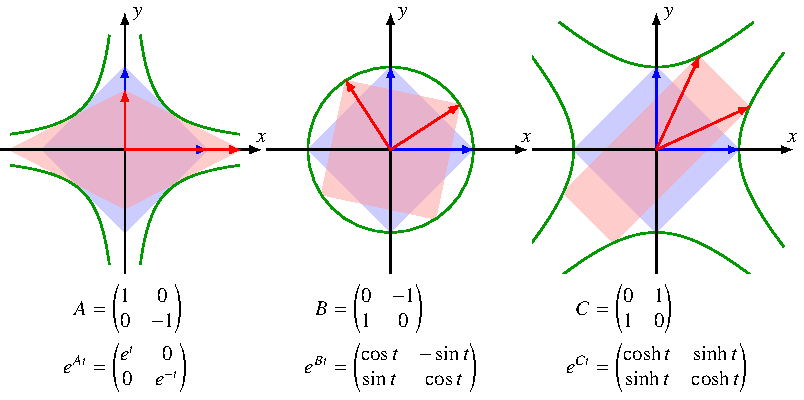
\includegraphics{chapters/60-gruppen/images/sl2.pdf}
\caption{Tangentialvektoren und die davon erzeugen Einparameteruntergruppen
für die Lie-Gruppe $\operatorname{SL}_2(\mathbb{R})$ der flächenerhaltenden
linearen Abbildungen von $\mathbb{R}^2$.
In allen drei Fällen wird ein blauer Rhombus mit den Ecken in den
Standardbasisvektoren von einer Matrix der Einparameteruntergruppe zu
zum roten Viereck verzerrt, der Flächeninhalt bleibt aber erhalten.
In den beiden Fällen $B$ und $C$ stellen die grünen Kurven die Bahnen
der Bilder der Standardbasisvektoren dar.
\label{buch:gruppen:fig:sl2}}
\end{figure}%
\begin{figure}
\centering
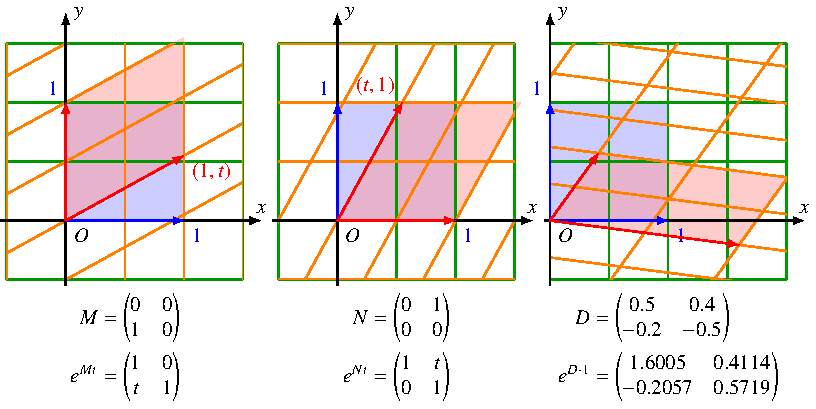
\includegraphics{chapters/60-gruppen/images/scherungen.pdf}
\caption{Weitere Matrizen mit Spur $0$ und ihre Wirkung 
Die inken beiden Beispiele $M$ und $N$ sind nilpotente Matrizen,
die zugehörigen Einparameter-Untergruppen beschreiben Schwerungen.
\label{buch:gruppen:fig:scherungen}}
\end{figure}
\end{beispiel}

%
% Die Gruppe SU(2)
%
\subsection{Die Gruppe $\operatorname{SU}(2)$
\label{buch:gruppen:su2}}
Die Menge der Matrizen
\[
\operatorname{SU}(2)
=
\left\{
\left.
A=\begin{pmatrix} a&b\\c&d\end{pmatrix}
\;\right|\;
a,b,c,d\in\mathbb{C},\det(A)=1, AA^*=I
\right\}
\]
heisst die {\em spezielle unitäre Gruppe}.
Wegen $\det(AB)=\det(A)\det(B)=1$ und $(AB)^*AB=B^*A^*AB=B^*B=I$ ist 
$\operatorname{SU}(2)$ eine Untergruppe von $\operatorname{GL}_2(\mathbb{C})$.
Die Bedingungen $\det A=1$ und $AA^*=I$ schränken die möglichen Werte
von $a$ und $b$ weiter ein.
Aus 
\[
A^*
=
\begin{pmatrix}
\overline{a}&\overline{c}\\
\overline{b}&\overline{d}
\end{pmatrix}
\]
und den Bedingungen führen die Gleichungen
\[
\begin{aligned}
a\overline{a}+b\overline{b}&=1
&&\Rightarrow&|a|^2+|b|^2&=1
\\
a\overline{c}+b\overline{d}&=0
&&\Rightarrow&
\frac{a}{b}&=-\frac{\overline{d}}{\overline{c}}
\\
c\overline{a}+d\overline{b}&=0
&&\Rightarrow&
\frac{c}{d}&=-\frac{\overline{b}}{\overline{a}}
\\
c\overline{c}+d\overline{d}&=1&&\Rightarrow&|c|^2+|d|^2&=1
\\
ad-bc&=1
\end{aligned}
\]
Aus der zweiten Gleichung kann man ableiten, dass es eine Zahl $t\in\mathbb{C}$
gibt derart, dass $c=-t\overline{b}$ und $d=t\overline{a}$.
Damit wird die Bedingung an die Determinante zu
\[
1
=
ad-bc = at\overline{a} - b(-t\overline{b})
=
t(|a|^2+|b|^2)
=
t,
\]
also muss die Matrix $A$ die Form haben
\[
A
=
\begin{pmatrix}
a&b\\
-\overline{b}&\overline{a}
\end{pmatrix}
\qquad\text{mit}\quad |a|^2+|b|^2=1.
\]
Schreibt man $a=a_1+ia_2$ und $b=b_1+ib_2$ mit rellen $a_i$ und $b_i$,
dann besteht $SU(2)$  aus den Matrizen der Form
\[
A=
\begin{pmatrix}
 a_1+ia_2&b_1+ib_2\\
-b_1+ib_2&a_1-ia_2
\end{pmatrix}
\]
mit der zusätzlichen Bedingung
\[
|a|^2+|b|^2
=
a_1^2 + a_2^2 + b_1^2 + b_2^2 = 1.
\]
Die Matrizen von $\operatorname{SU}(2)$ stehen daher in einer
eins-zu-eins-Beziehung zu den Vektoren $(a_1,a_2,b_1,b_2)\in\mathbb{R}^4$
eines vierdimensionalen reellen Vektorraums mit Länge $1$.
Geometrisch betrachtet ist also $\operatorname{SU}(2)$ eine dreidmensionalen
Kugel, die in einem vierdimensionalen Raum eingebettet ist.




%
% lie-algebren.tex -- Lie-Algebren
%
% (c) 2020 Prof Dr Andreas Müller, Hochschule Rapperswil
%
\section{Lie-Algebren
\label{buch:section:lie-algebren}}
\rhead{Lie-Algebren}
Im vorangegangenen Abschnitt wurde gezeigt, dass alle beschriebenen
Matrizengruppen als Untermannigfaltigkeiten im $n^2$-dimensionalen
Vektorraum $M_n(\mathbb{R})$ betrachtet werden können.
Die Gruppen haben damit nicht nur die algebraische Struktur einer
Matrixgruppe, sie haben auch die geometrische Struktur einer 
Mannigfaltigkeit.
Insbesondere ist es sinnvoll, von Ableitungen zu sprechen.

Eindimensionale Untergruppen einer Gruppe können auch als Kurven
innerhalb der Gruppe angesehen werden.
In diesem Abschnitt soll gezeigt werden, wie man zu jeder eindimensionalen
Untergruppe einen Vektor in $M_n(\mathbb{R})$ finden kann derart, dass
der Vektor als Tangentialvektor an diese Kurve gelten kann.
Aus einer Abbildung zwischen der Gruppe und diesen Tagentialvektoren
erhält man dann auch eine algebraische Struktur auf diesen Tangentialvektoren,
die sogenannte Lie-Algebra.
Sie ist charakteristisch für die Gruppe.
Insbesondere werden wir sehen, wie die Gruppen $\operatorname{SO}(3)$ 
und $\operatorname{SU}(2)$ die gleich Lie-Algebra haben und dass die
Lie-Algebra von $\operatorname{SO}(3)$ mit dem Vektorprodukt in $\mathbb{R}^3$
übereinstimmt.
\index{Vektorprodukt}%

%
% Die Lie-Algebra einer Matrizengruppe
%
\subsection{Lie-Algebra einer Matrizengruppe
\label{buch:section:lie-algebra-einer-matrizengruppe}}
Zu jedem Tangentialvektor $A$ im Punkt $I$ einer Matrizengruppe gibt es
eine Einparameteruntergruppe, die mit Hilfe der Exponentialfunktion
$e^{At}$ konstruiert werden kann.
Für die folgende Konstruktion arbeiten wir in der Gruppe
$\operatorname{GL}_n(\mathbb{R})$, in der jede Matrix auch ein
Tangentialvektor ist.
Wir werden daraus die Lie-Klammer ableiten und später verifizieren,
dass diese auch für die Tangentialvektoren der Gruppen
$\operatorname{SO}(n)$ oder $\operatorname{SL}_n(\mathbb{R})$ funktioniert.

\subsubsection{Lie-Klammer}
Zu zwei verschiedenen Tagentialvektoren $A\in M_n(\mathbb{R})$ und
$B\in M_n(\mathbb{R})$ gibt es zwei verschiedene Einparameteruntergruppen
$e^{At}$ und $e^{Bt}$.
Wenn die Matrizen $A$ und $B$ oder die Einparameteruntergruppen 
$e^{At}$ und $e^{Bt}$ vertauschbar sind, dann stimmen 
$e^{At}e^{Bt}$ und $e^{Bt}e^{At}$ nicht überein.
Die zugehörigen Potenzreihen sind:
\begin{align*}
e^{At}
&=
I+At + \frac{A^2t^2}{2!} + \frac{A^3t^3}{3!} + \dots
\\
e^{Bt}
&=
I+Bt + \frac{B^2t^2}{2!} + \frac{B^3t^3}{3!} + \dots
\\
e^{At}e^{Bt}
&=
\biggl(I+At + \frac{A^2t^2}{2!} + \dots\biggr)
\biggl(I+Bt + \frac{B^2t^2}{2!} + \dots\biggr)
\\
&=
I+(A+B)t + \biggl(\frac{A^2}{2!}+AB+\frac{B^2}{2!}\biggr)t^2 +\dots
\\
e^{Bt}e^{At}
&=
\biggl(I+Bt + \frac{B^2t^2}{2!} + \dots\biggr)
\biggl(I+At + \frac{A^2t^2}{2!} + \dots\biggr)
\\
&=
I+(B+A)t + \biggl(\frac{B^2}{2!}+BA+\frac{A^2}{2!}\biggr)t^2 +\dots
\intertext{%
Die beiden Kurven $e^{At}e^{Bt}$ und $e^{Bt}e^{At}$ haben zwar den gleichen
Tangentialvektor für $t=0$, sie unterscheiden
sich aber für $t>0$ und sie unterscheiden sich von der
Einparameteruntergruppe}
e^{(A+B)t}
&=
I + (A+B)t + \frac{t^2}{2}(A^2 + AB + BA + B^2) + \ldots
\intertext{von $A+B$. Für die Unterschiede finden wir}
e^{At}e^{Bt} - e^{(A+B)t}
&=
\biggl(AB-\frac{AB+BA}2\biggr)t^2
+\ldots
=
(AB-BA) \frac{t^2}{2} + \ldots
=
[A,B]\frac{t^2}{2}+\ldots
\\
e^{Bt}e^{At} - e^{(A+B)t}
&=
\biggl(BA-\frac{AB+BA}2\biggr)t^2
+\ldots
=
(BA-AB)
\frac{t^2}{2}
+\ldots
=
-[A,B]\frac{t^2}{2}
\\
e^{At}e^{Bt}-e^{Bt}e^{At}
&=
(AB-BA)t^2+\ldots
=
\phantom{-}[A,B]t^2+\ldots
\end{align*}
wobei $[A,B]=AB-BA$ abgekürzt wird.

\begin{definition}
\label{buch:gruppen:def:kommutator}
Der {\em Kommutator} zweier Matrizen $A,B\in M_n(\mathbb{R})$ ist die Matrix
$[A,B]=AB-BA$.
\index{Kommutator}%
\index{Lie-Klammer}%
\end{definition}

Der Kommutator ist bilinear und antisymmetrisch, da
\index{bilinear}%
\index{antisymmetrisch}%
\begin{align*}
[\lambda A+\mu B,C]
&=
\lambda AC+\mu BC-\lambda CA -\mu CB
=
\lambda[A,C]+\mu[B,C]
\\
[A,\lambda B+\mu C]
&=
\lambda AB + \mu AC - \lambda BA - \mu CA
=
\lambda[A,B]+\mu[A,C]
\\
[A,B]
&=
AB-BA = -(BA-AB) = -[B,A].
\end{align*}
Aus der letzten Bedingung folgt insbesodnere $[A,A]=0$

Der Kommutator $[A,B]$ misst in niedrigster Ordnung den Unterschied
zwischen den
$ e^{At} e^{Bt} $
und
$ e^{Bt} e^{At} $.
Der Kommutator der Tangentialvektoren $A$ und $B$ bildet also die
Nichtkommutativität der Matrizen $e^{At}$ und $e^{Bt}$ ab.

\subsubsection{Die Jacobi-Identität}
Der Kommutator hat die folgende zusätzliche algebraische Eigenschaft:
\begin{align*}
[A,[B,C]]
+
[B,[C,A]]
+
[C,[A,B]]
&=
[A,BC-CB]
+
[B,CA-AC]
+
[C,AB-BA]
\\
&=\phantom{+}
ABC-ACB-BCA+CBA
\\
&\phantom{=}+
BCA-BAC-CAB+ACB
\\
&\phantom{=}+
CAB-CBA-ABC+BAC
\\
&=0.
\end{align*}
Diese Eigenschaft findet man auch bei anderen Strukturen, zum Beispiel
bei Vektorfeldern, die man als Differentialoperatoren auf Funktionen 
betrachten kann.
Man kann dann einen Kommutator $[X,Y]$ für zwei Vektorfelder
$X$ und $Y$ definieren.
Dieser Kommutator von Vektorfeldern erfüllt ebenfalls die gleiche
Identität.

\begin{definition}
\label{buch:gruppen:def:jacobi}
Ein bilineares Produkt $[\;,\;]\colon V\times V\to V$ auf dem Vektorraum
erfüllt die {\em Jacobi-Identität}, wenn 
\index{Jacobi-Identität}%
\[
[u,[v,w]] + [v,[w,u]] + [w,[u,v]]=0
\]
ist für beliebige Vektoren $u,v,w\in V$.
\end{definition}

\subsubsection{Lie-Algebra}
Die Tangentialvektoren einer Lie-Gruppe tragen also mit dem Kommutator
eine zusätzliche Struktur, nämlich die Struktur einer Lie-Algebra.

\begin{definition}
Ein Vektorraum $V$ mit einem bilinearen, Produkt
\[
[\;,\;]\colon V\times V \to V : (u,v) \mapsto [u,v],
\]
welches zusätzlich die Jacobi-Identität~\ref{buch:gruppen:def:jacobi}
erfüllt, heisst eine {\em Lie-Algebra}.
\index{Lie-Algebra}%
\end{definition}

Die Lie-Algebra einer Lie-Gruppe $G$ wird mit $LG$ bezeichnet.
$LG$ besteht aus den Tangentialvektoren im Punkt $I$.
Die {\em Exponentialabbildung} $\exp\colon LG\to G:A\mapsto e^A$
\index{Exponentialabbildung}%
ist eine differenzierbare Abbildung von $LG$ in die Gruppe $G$.
Insbesondere kann die Inverse der Exponentialabbildung als eine
Karte in einer Umgebung von $I$ verwendet werden.

Für die Lie-Algebren der Matrizengruppen, die früher definiert worden
sind, verwenden wir die Notationskonvention, dass der Name der
Lie-Algebra der mit kleinen Buchstaben geschrieben Name der Lie-Gruppe ist.
Die Lie-Algebra von $\operatorname{SO}(n)$ ist also
$L\operatorname{SO}(n) = \operatorname{so}(n)$,
\index{so(n)@$\operatorname{so}(n)$}%
die Lie-Algebra von $\operatorname{SL}_n(\mathbb{R})$ ist
$L\operatorname{SL}_n(\mathbb{R})=\operatorname{sl}_n(\mathbb{R})$.
\index{sln(r)@$\operatorname{sl}_n(\mathbb{R})$}%

%
% Die Lie-Algebra von SO(3)
%
\subsection{Die Lie-Algebra von $\operatorname{SO}(3)$
\label{buch:subsection:die-lie-algebra-von-so3}}
Zur Gruppe $\operatorname{SO}(3)$ der Drehmatrizen gehört die Lie-Algebra
$\operatorname{so}(3)$ der antisymmetrischen $3\times 3$-Matrizen.
Solche Matrizen haben die Form
\[
\Omega
=
\begin{pmatrix}
    0    &-\omega_3& \omega_2\\
 \omega_3&   0     &-\omega_1\\
-\omega_2& \omega_1&    0
\end{pmatrix}
\]
Die antisymmetrischen Matrizen
\[
\omega_{23}
=
\begin{pmatrix} 0&0&0\\0&0&-1\\0&1&0\end{pmatrix},
\quad
\omega_{31}
=
\begin{pmatrix} 0&0&1\\0&0&0\\-1&0&0\end{pmatrix},
\quad
\omega_{12}
=
\begin{pmatrix} 0&1&0\\-1&0&0\\0&0&0\end{pmatrix}
\]
bilden eine Basis für $\operatorname{so}(3)$, man kann
\[
\Omega
=
\omega_1\omega_{23}
+
\omega_2\omega_{31}
+
\omega_3\omega_{12}
\]
schreiben.
Der Vektorraum $\operatorname{so}(3)$ ist also dreidimensional.

Die Kommutatoren der Basisvektoren sind
\begin{equation}
\setlength\arraycolsep{4pt}
\begin{aligned}
[\omega_{23},\omega_{31}]
&=
\begin{pmatrix}
0&-1&0\\
1&0&0\\
0&0&0
\end{pmatrix}
=
\omega_{12},
%\\
&
[\omega_{31},\omega_{12}]
&=
\begin{pmatrix}
0&0&0\\
0&0&-1\\
0&1&0
\end{pmatrix}
=
\omega_{23},
%\\
&
[\omega_{12},\omega_{23}]
&=
\begin{pmatrix}
0&0&1\\
0&0&0\\
-1&0&0
\end{pmatrix}
=
\omega_{31},
\end{aligned}
\label{buch:gruppen:eqn:so3-kommutatoren}
\end{equation}
wie man durch direkte Rechnung bestätigt.
Diese Regeln stimmen mit den Vektorprodukten der Standardbasisvektoren
in $\mathbb{R}^3$ überein.

\begin{figure}
\centering
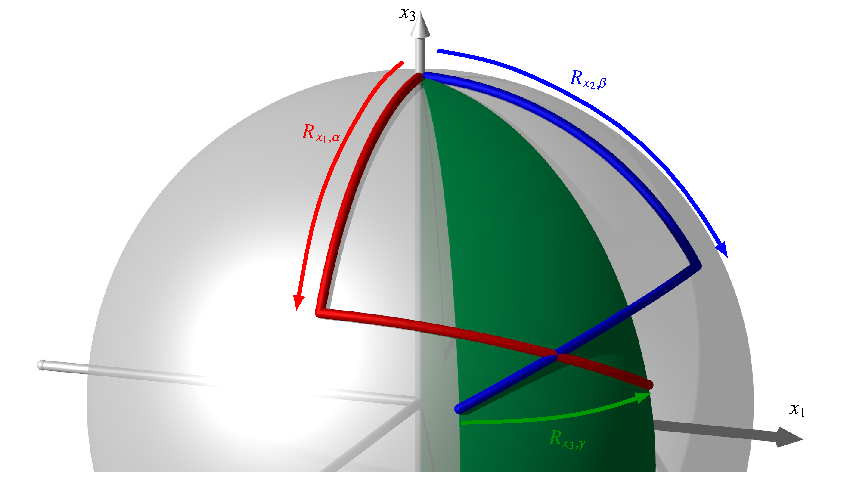
\includegraphics{chapters/60-gruppen/images/nichtkomm.pdf}
\caption{Der Kommutator zweier Drehungen um die $x_1$ und $x_2$
Achse ist eine Drehung um die $x_3$-Achse.
\label{buch:lie:fig:kommutator}}
\end{figure}
Abbildung~\ref{buch:lie:fig:kommutator} illustriert, wie der
Kommutator die Nichtkommutativität der Gruppe $\operatorname{SO}(3)$
wiedergibt.
Die Matrix $\omega_{23}$ erzeugt eine Drehung $R_{x_1,\alpha}$
um die $x_1$-Achse,
die Matrix $\omega_{31}$ eine Drehung $R_{x_2,\beta}$ um die $x_2$ Achse.
Der Kommutator $[\omega_{23},\omega_{31}]=\omega_{12}$ beschreibt in
niedrigster Ordnung den Unterschied, der entsteht, wenn man die
beiden Drehungen in verschiedenen Reihenfolgen ausführt.
Dies ist eine Drehung $R_{x_3,\gamma}$ um die $x_3$-Achse.

Aus der Rodriguez-Formel~\ref{buch:lie:eqn:rodrigues} wissen wir
bereits, dass die Ableitung der Drehung das Vektorprodukt
$\vec{\omega}\times\vec{x}$ ist.
Dieses kann jedoch auch als
$\Omega\vec{x} = \vec{omega}\times\vec{x}$
ausgedrückt werden.

Die Wirkung von $I+t\Omega$ auf einem Vektor $\vec{x}$ ist
\[
(I+t\Omega)
\begin{pmatrix}x_1\\x_2\\x_3\end{pmatrix}
=
\begin{pmatrix}
    1     &-t\omega_3& t\omega_2\\
 t\omega_3&   1      &-t\omega_1\\
-t\omega_2& t\omega_1&    1
\end{pmatrix}
\begin{pmatrix}x_1\\x_2\\x_3\end{pmatrix}
=
\begin{pmatrix}
x_1+t(-\omega_3x_2+\omega_2x_3)\\
x_2+t( \omega_3x_1-\omega_1x_3)\\
x_3+t(-\omega_2x_1+\omega_1x_2)
\end{pmatrix}
=
\vec{x}+ t\begin{pmatrix}\omega_1\\\omega_2\\\omega_3\end{pmatrix}\times x
=
\vec{x}+ t\vec{\omega}\times \vec{x}.
\]
Die Matrix $\Omega$ ist als die infinitesimale Version einer Drehung
um die Achse $\omega$.

Wir können die Analogie zwischen Matrizen in $\operatorname{so}(3)$ und
Vektoren in $\mathbb R^3$ noch etwas weiter treiben. Zu jedem Vektor
in $\mathbb R^3$ konstruieren wir eine Matrix in $\operatorname{so}(3)$
mit Hilfe der Abbildung
\[
\mathbb R^3\to\operatorname{so}(3)
:
\begin{pmatrix}v_1\\v_2\\v_3\end{pmatrix}
\mapsto
\begin{pmatrix}
  0 &-v_3& v_2\\
 v_3&  0 &-v_1\\
-v_2& v_1&  0
\end{pmatrix}.
\]
Der Kommutator von zwei so aus Vektoren $\vec u$ und $\vec v$
konstruierten Matrizen $U$ und $V$ ist:
\begin{align*}
[U,V]
&=
UV-VU
\\
&=
\begin{pmatrix}
  0 &-u_3& u_2\\
 u_3&  0 &-u_1\\
-u_2& u_1&  0
\end{pmatrix}
\begin{pmatrix}
  0 &-v_3& v_2\\
 v_3&  0 &-v_1\\
-v_2& v_1&  0
\end{pmatrix}
-
\begin{pmatrix}
  0 &-v_3& v_2\\
 v_3&  0 &-v_1\\
-v_2& v_1&  0
\end{pmatrix}
\begin{pmatrix}
  0 &-u_3& u_2\\
 u_3&  0 &-u_1\\
-u_2& u_1&  0
\end{pmatrix}
\\
&=
\begin{pmatrix}
-u_3v_3-u_2v_2 + u_3v_3 + u_2v_2
        & u_2v_1 - u_1v_2
                & u_3v_1 - u_1v_3
\\
u_1v_2 - u_2v_1
        & -u_3v_3-u_1v_1 + u_3v_3+u_1v_1
                & u_3v_2 - u_2v_3
\\
u_1v_3 - u_3v_1
        & u_2v_3 - u_3v_2
                &-u_2v_2-u_1v_1+ u_2v_2+u_1v_1
\end{pmatrix}
\\
&=
\begin{pmatrix}
0
        &-(u_1v_2 - u_2v_1)
                &u_3v_1-u_1v_3
\\
u_1v_2 - u_2v_1
        & 0
                &-(u_2v_3 - u_3v_2)
\\
-(u_3v_1 - u_1v_3)
        &   u_3v_2 - u_2v_3
                & 0
\end{pmatrix}.
\end{align*}
Die Matrix $[U,V]$ gehört zum Vektor $\vec u\times\vec v$.
Damit können wir aus der Jacobi-Identität jetzt folgern, dass
\[
\vec u\times(\vec v\times w)
+
\vec v\times(\vec w\times u)
+
\vec w\times(\vec u\times v)
=0
\]
für drei beliebige Vektoren $\vec u$, $\vec v$ und $\vec w$ ist.
Dies bedeutet, dass der dreidimensionale Vektorraum $\mathbb R^3$
mit dem Vektorprodukt zu einer Lie-Algebra wird.
In der Tat verwenden einige Lehrbücher statt der vertrauten Notation
$\vec u\times \vec v$ für das Vektorprodukt die aus der Theorie der
Lie-Algebren entlehnte Notation $[\vec u,\vec v]$, zum Beispiel
auch das Lehrbuch der Theoretischen Physik \cite{skript:landaulifschitz1}
von Landau und Lifschitz.

Die Lie-Algebren sind vollständig klassifiziert worden, es gibt
keine nicht trivialen zweidimensionalen Lie-Algebren.
Unser dreidimensionaler Raum ist also auch in dieser Hinsicht speziell:
es ist der kleinste Vektorraum, in dem eine nichttriviale Lie-Algebra-Struktur
möglich ist.

\subsection{Die Lie-Algebra von $\operatorname{SL}_n(\mathbb{R})$}
Die Lie-Algebra von $\operatorname{SL}_n(\mathbb{R})$ besteht aus den
spurlosen Matrizen in $M_n(\mathbb{R})$.
Der Kommutator solcher Matrizen erfüllt
\[
\operatorname{Spur}([A,B])
=
\operatorname{Spur}(AB-BA)
=
\operatorname{Spur}(AB)-\operatorname{Spur}(BA)
=
0,
\]
somit ist 
\[
\operatorname{sl}_n(\mathbb{R})
=
\{
A\in M_n(\mathbb{R})\;|\; \operatorname{Spur}(A)=0
\}
\]
mit dem Kommutator eine Lie-Algebra.

%
% Die Lie-Algebra von U(n)
%
\subsection{Die Lie-Algebra von $\operatorname{U}(n)$}
Die Lie-Gruppe
\[
U(n)
=
\{
A\in M_n(\mathbb{C}
\;|\;
AA^*=I
\}
\]
\index{unitäre Gruppe}%
\index{Gruppe, unitär}%
\index{U(n)@$\operatorname{U}(n)$}%
heisst die unitäre Gruppe, sie besteht aus den Matrizen, die
das sesquilineare Standardskalarprodukt auf dem komplexen
Vektorraum $\mathbb{C}^n$ invariant lassen.
Sei eine $\gamma(t)$ ein differenzierbare Kurve in $\operatorname{U}(n)$
derart, dass $\gamma(0)=I$.
Die Ableitung der Identität $AA^*=I$ führt dann auf 
\begin{equation*}
0
=
\frac{d}{dt}
\gamma(t)\gamma(t)^*
\bigg|_{t=0}
=
\dot{\gamma}(0)\gamma(0)^*
+
\gamma(0)\dot{\gamma}(0)^*
=
\dot{\gamma}(0)
+
\dot{\gamma}(0)^*
\quad\Rightarrow\quad
\dot{\gamma}(0)=-\dot{\gamma}(0)^*
\quad\Rightarrow\quad
A=-A^*
\end{equation*}
Die Lie-Algebra $\operatorname{u}(n)$ besteht daher aus den antihermiteschen
Matrizen.
\index{u(n)@$\operatorname{u}(n)$}%

Wir sollten noch verifizieren, dass der Kommutator zweier antihermiteschen
Matrizen wieder anithermitesch ist:
\index{antihermitesch}%
\begin{align*}
[A,B]^*
&=
(AB-BA)^*
=
B^*A^*-A^*B^*
=
BA - AB
=
-[B,A].
\end{align*}

Eine antihermitesche Matrix erfüllt $a_{i\!j}=-\overline{a}_{ji}$,
für die Diagonalelemente folgt daher $a_{ii} = -\overline{a}_{ii}$
oder $\overline{a}_{ii}=-a_{ii}$.
Der Realteil von $a_{ii}$ ist
\[
\Re a_{ii}
=
\frac{a_{ii}+\overline{a}_{ii}}2
=
0,
\]
die Diagonalelemente einer antihermiteschen Matrix sind daher rein
imaginär.


%
% Die Lie-Algebra SU(2)
%
\subsection{Die Lie-Algebra von $\operatorname{SU}(2)$}
Die Lie-Algebra $\operatorname{su}(n)$ besteht aus den
spurlosen antihermiteschen Matrizen.
\index{su(n)@$\operatorname{su}(n)$}%
Sie erfüllen daher die folgenden Bedingungen:
\[
A=\begin{pmatrix}a&b\\c&d\end{pmatrix}
\qquad
\text{mit}
\qquad
\left\{
\begin{aligned}
a+d&=0&&\Rightarrow& a=is = -d
\\
b^*&=-c
\end{aligned}
\right.
\]
Damit hat $A$ die Form
\begin{align*}
A=\begin{pmatrix}
is&u+iv\\
-u+iv&-is
\end{pmatrix}
&=
s
\begin{pmatrix}
i&0\\
0&-i
\end{pmatrix}
+
u
\begin{pmatrix}
 0&1\\
-1&0
\end{pmatrix}
+
v
\begin{pmatrix}
0&i\\
i&0
\end{pmatrix}
\\
&=
iv\underbrace{\begin{pmatrix}0&1\\1&0\end{pmatrix}}_{\displaystyle=\sigma_1}
+
iu\underbrace{\begin{pmatrix}0&-i\\i&0\end{pmatrix}}_{\displaystyle=\sigma_2}
+
is\underbrace{\begin{pmatrix}1&0\\0&-1\end{pmatrix}}_{\displaystyle=\sigma_3}
\end{align*}
Diese Matrizen heissen die {\em Pauli-Matrizen}, sie haben die Kommutatoren
\index{Pauli-Matriizen}%
\begin{align*}
[\sigma_1,\sigma_2]
&=
\begin{pmatrix}0&1\\1&0\end{pmatrix}
\begin{pmatrix}0&-i\\i&0\end{pmatrix}
-
\begin{pmatrix}0&-i\\i&0\end{pmatrix}
\begin{pmatrix}0&1\\1&0\end{pmatrix}
=
2\begin{pmatrix}i&0\\0&-i \end{pmatrix}
=
2i\sigma_3,
\\
[\sigma_2,\sigma_3]
&=
\begin{pmatrix}0&-i\\i&0\end{pmatrix}
\begin{pmatrix}1&0\\0&-1\end{pmatrix}
-
\begin{pmatrix}1&0\\0&-1\end{pmatrix}
\begin{pmatrix}0&-i\\i&0\end{pmatrix}
=
2
\begin{pmatrix}0&i\\i&0\end{pmatrix}
=
2i\sigma_1.
\\
[\sigma_1,\sigma_3]
&=
\begin{pmatrix}0&1\\1&0\end{pmatrix}
\begin{pmatrix}1&0\\0&-1\end{pmatrix}
-
\begin{pmatrix}1&0\\0&-1\end{pmatrix}
\begin{pmatrix}0&1\\1&0\end{pmatrix}
=
2i
\begin{pmatrix}0&-1\\1&0\end{pmatrix}
=
2i\sigma_2,
\end{align*}
Bis auf eine Skalierung stimmt dies überein mit den Kommutatorprodukten
der Matrizen $\omega_{23}$, $\omega_{31}$ und $\omega_{12}$
in \eqref{buch:gruppen:eqn:so3-kommutatoren}.
Die Matrizen $-\frac12i\sigma_j$ haben die Kommutatorprodukte
\begin{align*}
\bigl[-{\textstyle\frac12}i\sigma_1,-{\textstyle\frac12}i\sigma_2\bigr]
&=
-{\textstyle\frac14}[\sigma_1,\sigma_2]
=
-{\textstyle\frac14}\cdot 2i\sigma_3
=
-{\textstyle\frac12}i\sigma_3
\\
\bigl[-{\textstyle\frac12}i\sigma_2,-{\textstyle\frac12}i\sigma_3\bigr]
&=
-{\textstyle\frac14}[\sigma_2,\sigma_3]
=
-{\textstyle\frac14}\cdot 2i\sigma_1
=
-{\textstyle\frac12}i\sigma_1
\\
\bigl[-{\textstyle\frac12}i\sigma_3,-{\textstyle\frac12}i\sigma_1\bigr]
&=
-{\textstyle\frac14}[\sigma_3,\sigma_1]
=
-{\textstyle\frac14}\cdot 2i\sigma_2
=
-{\textstyle\frac12}i\sigma_2.
\end{align*}
Die lineare Abbildung, die
\begin{align*}
\omega_{23}&\mapsto -{\textstyle\frac12}i\sigma_1\\
\omega_{31}&\mapsto -{\textstyle\frac12}i\sigma_2\\
\omega_{12}&\mapsto -{\textstyle\frac12}i\sigma_3
\end{align*}
abbildet, ist daher ein Isomorphismus der Lie-Algebra $\operatorname{so}(3)$
auf die Lie-Algebra $\operatorname{su}(2)$.
Die Lie-Gruppen $\operatorname{SO}(3)$ und $\operatorname{SU}(2)$
haben also die gleiche Lie-Algebra.

Tatsächlich kann man Hilfe von Quaternionen die Matrix $\operatorname{SU}(2)$
als Einheitsquaternionen beschreiben und damit eine Darstellung der
Drehmatrizen in $\operatorname{SO}(3)$ finden.
Dies wird in Kapitel~\ref{chapter:clifford} dargestellt.






%%
% homogen.tex -- disktrete Untergruppen, homogene Räume
%
% (c) 2020 Prof Dr Andreas Müller, Hochschule Rapperswil
%
\section{Homogene Räume
\label{section:homogene-raeume}}


\section*{Übungsaufgaben}
\rhead{Übungsaufgaben}
\aufgabetoplevel{chapters/60-gruppen/uebungsaufgaben}
\begin{uebungsaufgaben}
\uebungsaufgabe{6002}
\uebungsaufgabe{6001}
\end{uebungsaufgaben}

